\documentclass{article}

\usepackage{float}
\usepackage[a4paper, total={6in, 8in}]{geometry}
\usepackage{fancyhdr}
\usepackage{graphicx}
\usepackage{amsmath}
\usepackage{amsfonts}
\usepackage{amssymb}
\usepackage{amsthm}
\usepackage[utf8]{inputenc}
\usepackage[T1]{fontenc}
\usepackage[french]{babel}
\usepackage{libertine}
\usepackage{listings}
\usepackage{color}
\usepackage[table]{xcolor}
\usepackage{minted}
\usepackage{hyperref}
\usepackage{csquotes}
\usepackage{url}
\usepackage[
    backend=biber,
    style=alphabetic,
    sorting=ynt
    ]{biblatex}
\addbibresource{references.bib}

\usepackage[center]{caption}
\hypersetup{
    colorlinks=true,
    pdftitle={PFE - Pluie en Australie},
    }
    
\begin{document}

\newcommand{\HRule}{\rule{\linewidth}{0.5mm}}

\begin{titlepage}
  \begin{sffamily}
  \begin{center}
    \hfill
    
\includegraphics[scale=0.06]{./Images/logoINSARouen.png}~\\[1.5cm]

    \textsc{\LARGE INSA ROUEN}\\[1cm]

    \textsc{\Large Projet de Fin d'Études}\\[1cm]

    \HRule \\[0.4cm]
    { \huge \bfseries Pluie en Australie\\[0.4cm] }

    \HRule \\[1cm]
    %\includegraphics[width=0.7\textwidth]{Ressources/front.pdf}
    %\\[1cm]

    \begin{minipage}{0.4\textwidth}
      \begin{flushleft} \large
        Théophile THIERRY\\
      \end{flushleft}
    \end{minipage}
    \begin{minipage}{0.4\textwidth}
      \begin{flushright} \large
        \textsc{M. PORTIER}\\
         2021-2022\\
      \end{flushright}
    \end{minipage}

    \vfill

  \end{center}
  \end{sffamily}
\end{titlepage}

\tableofcontents
\newpage

\part{Description des données}

\section{Présentation des données}

Les données utilisées pour ce projet peuvent être trouvées sur le site \href{https://www.kaggle.com/jsphyg/weather-dataset-rattle-package}{Kaggle}. Elles ont été récupérées des données du gouvernement australien, dans la partie \href{http://www.bom.gov.au/climate/dwo}{Daily Weather Observations}, et ont été complétées avec les données de la partie :  \href{http://www.bom.gov.au/climate/data}{Climate Data Online}.

Ces données contient 10 années d'observations de la météo australienne sur 49 lieux différents entre 2007 et 2017. Une observation est constituée de (presque) toutes ces variables : 

\begin{itemize}
    \item Date : date de la mesure.
    \item Location : localisation de la mesure.
    \item MinTemp : température minimale dans les 24h jusqu'à 9h du matin (en °C).
    \item MaxTemp : température maximale dans les 24h jusqu'à 9h du matin (en °C).
    \item Rainfall : précipitation dans les 24h jusqu'à 9h du matin (en mm).
    \item Evaporation : bac d'évaporation de classe A dans les 24h jusqu'à 9h du matin (en mm).
    \item Sunshine : ensoleillement en heure dans les 24h jusqu'à minuit.
    \item WindGustDir : direction de la plus forte rafale dans les 24 heures jusqu'à minuit (16 points cardinaux/intercardinaux).   
    \item WindGustSpeed : vitesse de la plus forte rafale dans les 24 heures jusqu'à minuit (16 points cardinaux/intercardinaux).
    \item WindDir9am : direction du vent à 9h du matin.
    \item WindDir3pm : idem à 15h.
    \item WindSpeed9am : vitesse du vent à 9h.
    \item WindSpeed3pm : idem à 15h.
    \item Humidity9am : taux d'humidité relative à 9h.
    \item Humidity3pm : idem à 15h.
    \item Pressure9am : pression atmosphérique réduite au niveau moyen de la mer à 9h.
    \item Pressure3pm : idem à 15h.
    \item Cloud9am : fraction du ciel couverte par un nuage à 9h (en huitième).   
    \item Cloud3pm : idem à 15h.
    \item Temp9am : température à 9h (en °C).
    \item Temp3pm : idem à 15h.
    \item RainToday : s'il a plu le jour même.
    \item RainTomorrow : s'il a plu le lendemain.   
\end{itemize}

Jetons tout d'abord un coup d'oeil aux variables numériques de nos données. 

\subsection{Variables numériques}

\begin{table}[ht]
    \centering
    \resizebox{\textwidth}{!}{
        \begin{tabular}{|r||rrrrrrrr|}
            \hline
            & Min. & 1st Qu. & Median & Mean & 3rd Qu. & Max. & NA's & Std. \\ 
            \hline
            \hline
            MinTemp & -8.50 & 7.60 & 12.00 & 12.19 & 16.90 & 33.90 & 1485.00 & 6.40 \\ 
            MaxTemp & -4.80 & 17.90 & 22.60 & 23.22 & 28.20 & 48.10 & 1261.00 & 7.12 \\ 
            Rainfall & 0.00 & 0.00 & 0.00 & 2.36 & 0.80 & 371.00 & 3261.00 & 8.48 \\ 
            Evaporation & 0.00 & 2.60 & 4.80 & 5.47 & 7.40 & 145.00 & 62790.00 & 4.19 \\ 
            Sunshine & 0.00 & 4.80 & 8.40 & 7.61 & 10.60 & 14.50 & 69835.00 & 3.79 \\ 
            WindGustSpeed & 6.00 & 31.00 & 39.00 & 40.04 & 48.00 & 135.00 & 10263.00 & 13.61 \\ 
            WindSpeed9am & 0.00 & 7.00 & 13.00 & 14.04 & 19.00 & 130.00 & 1767.00 & 8.92 \\ 
            WindSpeed3pm & 0.00 & 13.00 & 19.00 & 18.66 & 24.00 & 87.00 & 3062.00 & 8.81 \\ 
            Humidity9am & 0.00 & 57.00 & 70.00 & 68.88 & 83.00 & 100.00 & 2654.00 & 19.03 \\ 
            Humidity3pm & 0.00 & 37.00 & 52.00 & 51.54 & 66.00 & 100.00 & 4507.00 & 20.80 \\ 
            Pressure9am & 980.50 & 1012.90 & 1017.60 & 1017.65 & 1022.40 & 1041.00 & 15065.00 & 7.11 \\ 
            Pressure3pm & 977.10 & 1010.40 & 1015.20 & 1015.26 & 1020.00 & 1039.60 & 15028.00 & 7.04 \\ 
            Cloud9am & 0.00 & 1.00 & 5.00 & 4.45 & 7.00 & 9.00 & 55888.00 & 2.89 \\ 
            Cloud3pm & 0.00 & 2.00 & 5.00 & 4.51 & 7.00 & 9.00 & 59358.00 & 2.72 \\ 
            Temp9am & -7.20 & 12.30 & 16.70 & 16.99 & 21.60 & 40.20 & 1767.00 & 6.49 \\ 
            Temp3pm & -5.40 & 16.60 & 21.10 & 21.68 & 26.40 & 46.70 & 3609.00 & 6.94 \\ 
                \hline
        \end{tabular}
    }
    \caption{Résumé des variables numériques}
    \label{table:summary}
\end{table}

Comme nous pouvons le constater dans la Table \ref{table:summary}, pour certaines d'entre elles, il manque beaucoup d'observations (voir la ligne \emph{NA's}). Nous allons devoir remédier à cela dans les futures parties, et principalement sur les variables \emph{Sunshine}, \emph{Evaporation}, \emph{Cloud9am} et \emph{Cloud3pm}, dont nous avons moins de 60\% des observations.

Nous pouvons de plus noter certaines choses : comme on pouvait s'y attendre, il fait en général moins froid à 15h qu'à 9h, et il fait aussi moins humide. 

\subsection{Variables factorielles}

\begin{figure}[H]
    \centering
    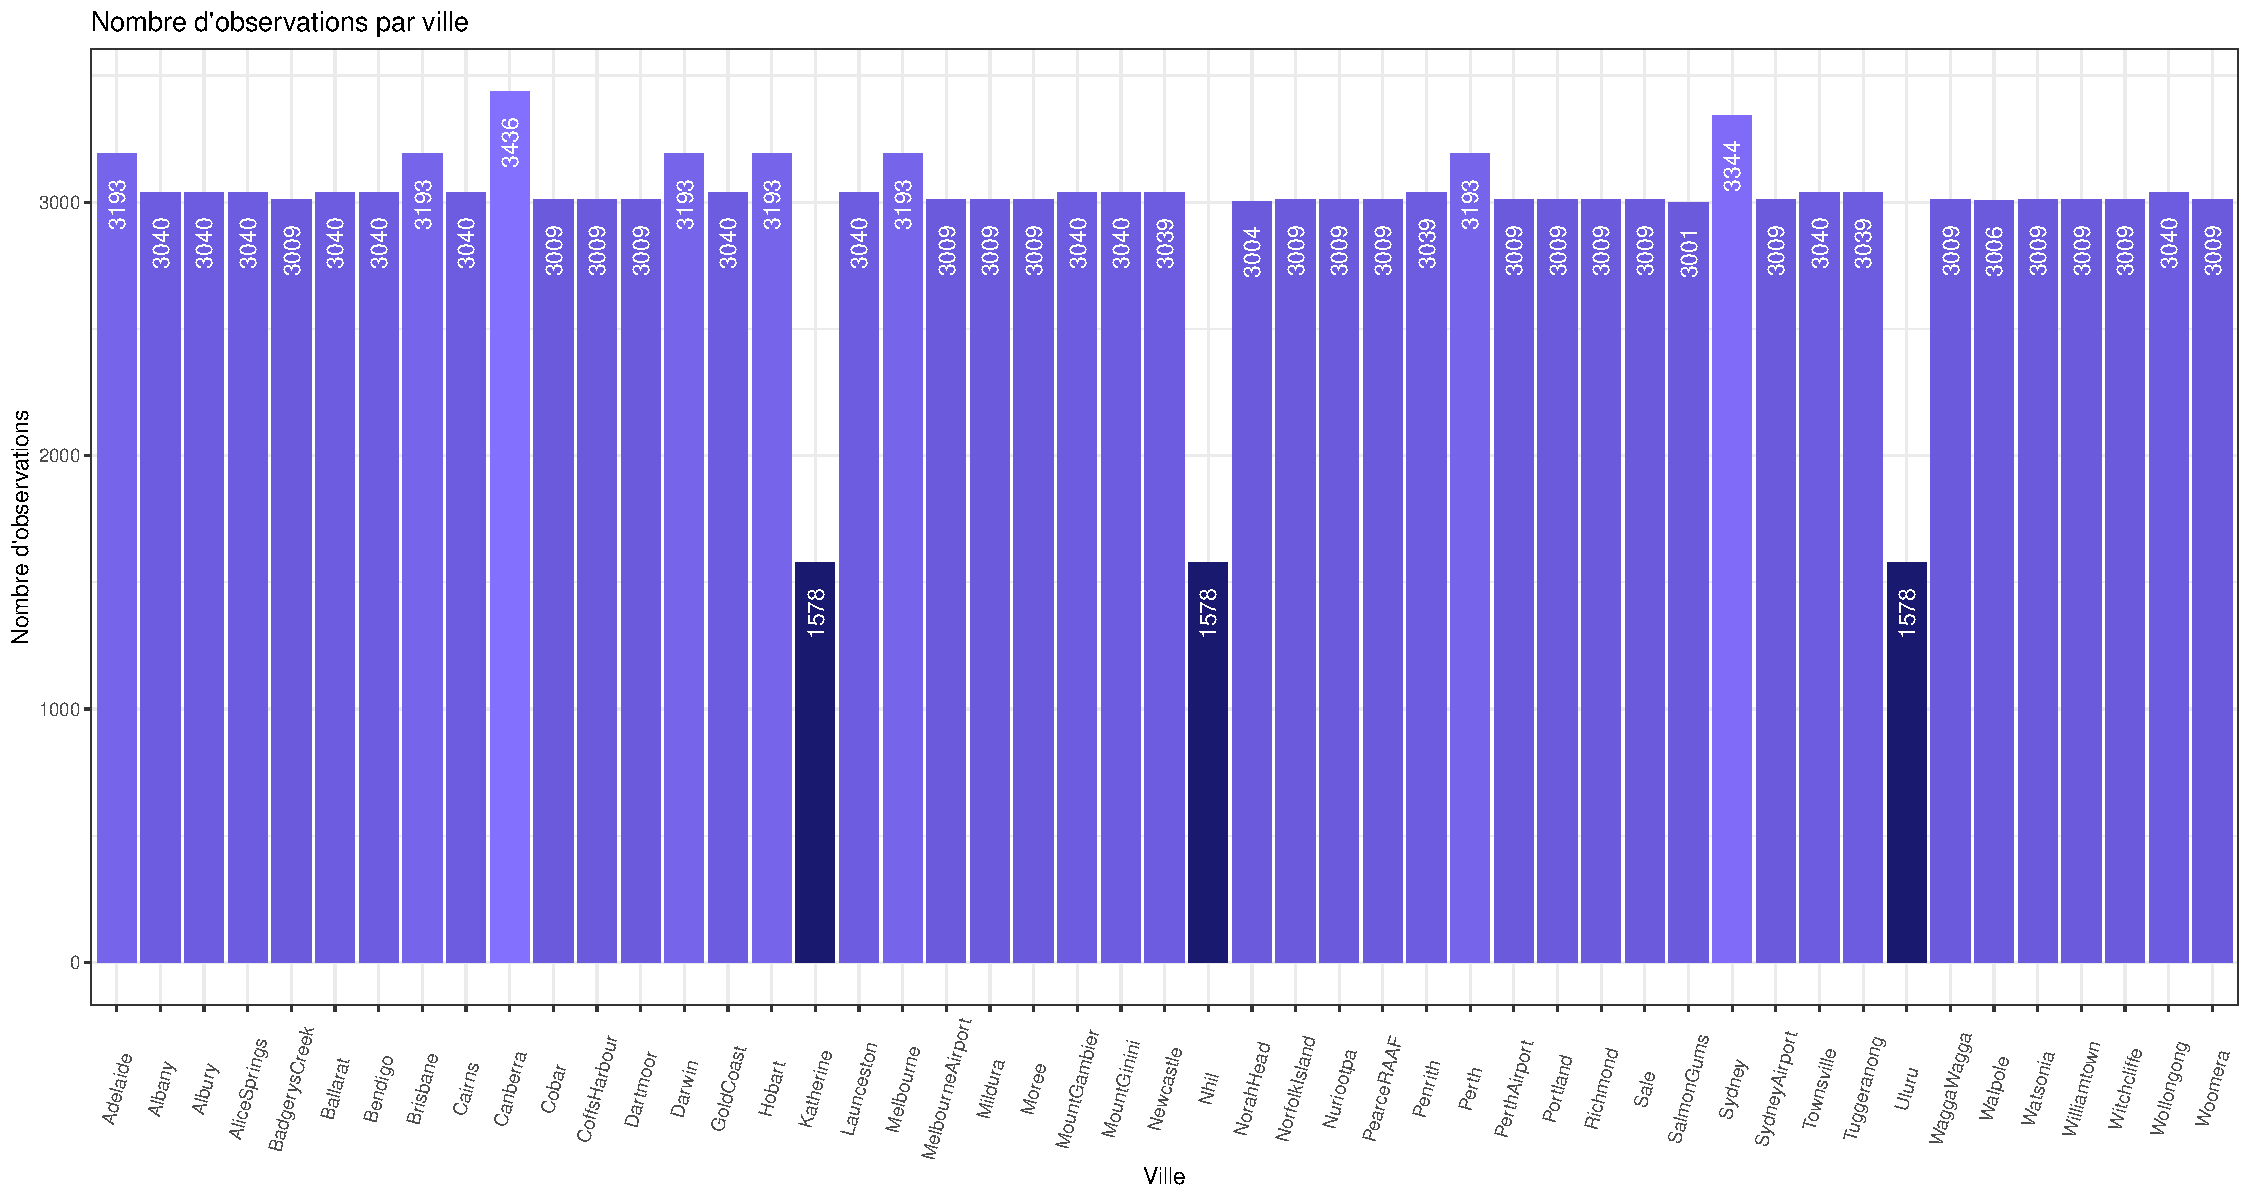
\includegraphics[width=\textwidth]{Images/hist_observations_cities.pdf}
    \caption{Nombre d'observations pour chaque ville}
    \label{fig:obs_per_cities}
\end{figure}

Regardons désormais les variables avec des facteurs. Les dates, tout d'abord, vont du 2007-11-01 au 2017-06-25, ce qui représente 3524 jours. Si l'on regarde la distribution du nombre d'observations par ville, on devrait donc voir que chacune d'entre elles en ont 3524 (voir Figure \ref{fig:obs_per_cities}). On voit déjà qu'il manque certaines dates d'observations pour la plupart des villes, et pour 3 d'entre elles : Katherine, Nhil et Uluru, nous avons moins de la moitié. Ceci est dû au fait que les observations démarrent à ces endroits en 2013.

Penchons-nous désormais sur les variables de direction du vent en regardant la distribution de leur facteurs dans les Tables \ref{table:wind_gust_dir}, \ref{table:wind_dir_9am} et \ref{table:wind_dir_3pm}.

\begin{table}[p]
    \centering
    \resizebox{\textwidth}{!}{
        \begin{tabular}{|r||*{17}{r}|}
            \hline
            & E & ENE & ESE & N & NE & NNE & NNW & NW & S & SE & SSE & SSW & SW & W & WNW & WSW & NA's \\
            \hline
            \hline
            Compte & 9181 & 8104 & 7372 & 9313 & 7133 & 6548 & 6620 & 8122 & 9168 & 9418 & 9216 & 8736 & 8967 & 9915 & 8252 & 9069 & 10326 \\
            \% & 6.31 & 5.57 & 5.07 & 6.40 & 4.90 & 4.50 & 4.55 & 5.58 & 6.30 & 6.47 & 6.34 & 6.01 & 6.16 & 6.82 & 5.67 & 6.23 & 7.10 \\
            \hline
        \end{tabular}
    }
    \caption{Variable WindGustDir}
    \label{table:wind_gust_dir}
\end{table}

\begin{table}[p]
    \centering
    \resizebox{\textwidth}{!}{
        \begin{tabular}{|r||*{17}{r}|}
            \hline
            & E & ENE & ESE & N & NE & NNE & NNW & NW & S & SE & SSE & SSW & SW & W & WNW & WSW & NA's \\
            \hline
            \hline
            Compte & 9176 & 7836 & 7630 & 11758 & 7671 & 8129 & 7980 & 8749 & 8659 & 9287 & 9112 & 7587 & 8423 & 8459 & 7414 & 7024 & 10566  \\
            \% & 6.31 & 5.39 & 5.25 & 8.08 & 5.27 & 5.59 & 5.49 & 6.01 & 5.95 & 6.38 & 6.26 & 5.22 & 5.79 & 5.82 & 5.10 & 4.83 & 7.26 \\
            \hline
        \end{tabular}
    }
    \caption{Variable WindDir9am}
    \label{table:wind_dir_9am}
\end{table}
 
\begin{table}[p]
    \centering
    \resizebox{\textwidth}{!}{
        \begin{tabular}{|r||*{17}{r}|}
            \hline
            & E & ENE & ESE & N & NE & NNE & NNW & NW & S & SE & SSE & SSW & SW & W & WNW & WSW & NA's \\
            \hline
            \hline
            Compte & 8472 & 7857 & 8505 & 8890 & 8263 & 6590 & 7870 & 8610 & 9926 & 10838 & 9399 & 8156 & 9354 & 10110 & 8874 & 9518 & 4228   \\
            \% & 5.82 & 5.40 & 5.85 & 6.11 & 5.68 & 4.53 & 5.41 & 5.92 & 6.82 & 7.45 & 6.46 & 5.61 & 6.43 & 6.95 & 6.10 & 6.54 & 2.91 \\
            \hline
        \end{tabular}
    }
    \caption{Variable WindDir3pm}
    \label{table:wind_dir_3pm}
\end{table}

Les 16 niveaux utilisés pour ces variables sont tous représentés avec à peu près la même distribution. Nous souhaitons changer ces facteurs en valeurs numériques, pour cela, nous allons remplacer chaque direction par sa valeur en degrés : utiliser l'angle pour la directions nous servira peut-être lorsque nous utiliserons des modèles de prédiction comme des arbres CART. En effet, baisser le nombre de facteurs que nous avons nous permettra sûrement de réduire le nombre de feuilles que nous aurions pu avoir. Nous utiliserons les valeurs indiquée dans la Table \ref{table:deg}.

\begin{table}[H]
    \centering
    \resizebox{\textwidth}{!}{
        \begin{tabular}{|r||*{16}{r}|}
            \hline
            & E & ENE & ESE & N & NE & NNE & NNW & NW & S & SE & SSE & SSW & SW & W & WNW & WSW \\
            \hline
            Degré & 0.0 & 22.5 & 45.0 & 67.5 & 90.0 & 112.5 & 135.0 & 157.5 & 180.0 & 202.5 & 225.0 & 247.5 & 270.0 & 292.5 & 315.0 & 337.5 \\
            \hline
        \end{tabular}
    }
    \caption{Les 16 points cardinaux en degrés}
    \label{table:deg}
\end{table}

On remarque une fois de plus qu'une partie de ses observations sons manquantes (plus de 7\% pour \emph{WindGustDir} et \emph{WindDir9am} et un peu moins de 3\% pour \emph{WindDir3pm})


\begin{table}[p]
    \centering
    \begin{tabular}{|r||rrr|}
        \hline
        &    No &    Yes &   NA's \\
        \hline
        \hline
        Compte & 110319 &  31880 &   3261 \\
        \% & 75.84 & 21.92 & 2.24 \\
        \hline
    \end{tabular}
    \caption{Variable RainToday}
    \label{table:rain_today}
\end{table}

\begin{table}[p]
    \centering
    \begin{tabular}{|r||rrr|}
        \hline
        &    No &    Yes &   NA's \\
        \hline
        \hline
        Compte & 110316 &  31877 &   3267 \\
        \% & 75.84 & 21.91 & 2.25 \\
        \hline
    \end{tabular}
    \caption{Variable RainTomorrow}
    \label{table:rain_tomorrow}
\end{table}

Enfin, nous avons les deux dernières variables booléennes concernant la pluie (Tables \ref{table:rain_today} et \ref{table:rain_tomorrow}). On voit que notre base de données est déséquilibrée : la variable que nous voulons prédire étant \emph{RainTomorrow}, nous voulons avoir une équilibre entre les observations \emph{Yes} et les observations \emph{No}. Pour veiller à ceci, nous utiliserons des méthodes de resampling telle que SMOTE. 

On remarque de plus que nous avons ~2.25\% des variables manquantes pour ces deux variables. Ceci s'explique par le fait qu'il manque ~2.25\% des observations de la variable \emph{Rainfall}, sur laquelle sont basées ces deux variables.

Enfin, nous avons la variables \emph{Location} qui contient tous les lieux d'observations de la base de données. Nous nous pencherons sur celle-ci dans la section Cartographie. 

Avant de nous lancer plus loin, nous allons tout d'abord modifier la base de données pour la rendre utilisable. Pour cela, nous devons nous occuper des variables qui contiennent des facteurs et les changer en numériques, comme nous avons fait pour les variables de direciton du vent. Nous allons ensuite remplacer la variable lieu avec une variable de longitude et de latitude, pour des raisons que nous expliquerons dans la section suivante. Enfin, nous allons rajouter une variable correspondant aux climats de chaque lieu (on prendra pour cela une carte des climats et on pourra rentrer à la main chaque climat de chaque lieu). Pour ce qui est de la variable date, nous la remplacerons par une variable saison à seulement 4 niveaux. Ce choix sera expliqué dans une partie sur le climat et sur les périodicités. Au final, nous pourrons nous occuper du traitement des observations manquantes. 

\section{Cartographie}

Notre base de donnée comprend donc une variable \emph{Location}, qui est une variable qualitative avec le nom du lieu de mesure. Nous en avons 49 différentes, et afin de visualiser un peu mieux ces différents points d'observation, nous voulons les afficher sur une carte. 

Pour cela, nous allons utiliser le paquet R "rnaturalearth", qui nous offre un moyen simple de dessiner nos propres cartes en utilisant le standard WGS84 (World Geodetic System).

\subsection{Un standard de localisation et une projection}

Afin de localiser avec précision un point sur Terre, nous avons besoin d'un standard de localisation. Un standard est basé sur un système de coordonnées géodésique. Il peut utiliser notamment un système de coordonnées en Longitude et Latitude.

\subsubsection{Latitude et Longitude}

Afin d'avoir une coordonnée pour n'importe quel point sur Terre, nous utilisons des coordonnées de Longitude et de Latitude. Ce sont des valeurs exprimées en degré à partir d'un degré 0 de référence.

La Terre ne peut être représentée comme une sphère car cela rendrait les coordonnées trop imprécises par rapport à la réalité. Elle est de plus arrondie aux pôles et c'est pour ces raisons que nous représentons la Terre par un éllipsoïde. 

La Longitude est une coordonnée géographique représentée par une valeur angulaire, expression du positionnement est-ouest d'un point sur Terre \cite{frwiki:188614923}. Tous les points étant situés sur une courbure de l'élipsoïde reliant les pôle Nord et Sud et traversant l'équateur     perpendiculairement ont la même longitude. Une courbure de référence, appelé "méridien" est choisi arbitrairement (le méridien de Greenwich) comme degré 0. Les valeurs de Longitude s'étendent de -180° vers l'ouest à 180° à l'est par rapport à ce méridien. 

La Latitude est une coordonnée similaire mais qui à pour plan de référence l'équateur. Tous les points sur Terre ayant une même latitude forment un cercle dont le plan est parallèle à celui de l'équateur \cite{frwiki:189341688}. 

\begin{figure}[H]
    \centering
    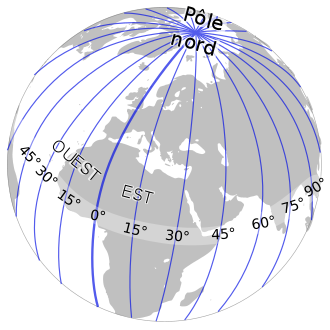
\includegraphics[width=0.3\textwidth]{Images/Cartographie/Longitude.png}
    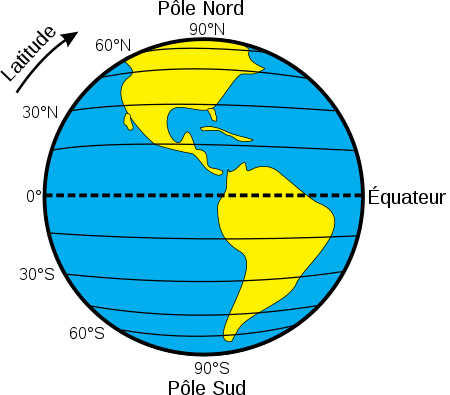
\includegraphics[width=0.3\textwidth]{Images/Cartographie/Latitude.png}
    \caption{Illustration du système de coordonnées de Longitude et Latitude}
\end{figure}

Lorsque l'on combine ce système de coordonnées et une représentation de la Terre en ellipsoïde (au travers de mesures précises des dimensions de la planète), on obtient un système géodésique.

\subsubsection{Le WSG84}

Le World Geodetic System 84 (WGS84) est un système géodésique, et nous pouvons l'utiliser pour nos cartes grâce au paquet "rnaturalearth". Il est notamment utilisé par le système GPS (Global Positioning System). Ce standard à été établi et est maintenu par le National Geospatial Intelligence Agency (NGA) des Etats-Unis \cite{enwiki:1065796786} depuis 1984. Il est basé sur un ellipsoïde de référence raffiné avec le temps pour représenter au mieux la Terre, ainsi que le système de coordonnées en Longitude et Latitude.

Nous avons maintenant un moyen de localiser précisément un point sur Terre grâce à deux valeurs numériques. Pour pouvoir les afficher sur une carte, il nous faut cependant une projection.

\subsubsection{Projections}

La projection cartographique est "un ensemble de techniques permettant de représenter la surface de la Terre dans son ensemble ou en partie sur la surface plane d'une carte" \cite{frwiki:181713838}. La Terre étant sphérique, afin de l'afficher sur une carte plane, il faut la projeter. Il existe différent types de projections, certaines permettent de conserver localement les surfaces, d'autres les angles ou encore les distances sur les méridiens. 

Notre paquet utilise de base une projection dite géographique : elle consiste simplement à prendre les valeurs de latitude et de longitude et des les utiliser comme si elles étaient les coordonnées X et Y (respectivement) d'un repère en deux dimensions. Cette "projection" peut avoir des résultats différents en fonction du système géodésique utilisé. 

Le plus gros inconvénient de cette pratique est la distorsion des surfaces lorsque l'on s'éloigne de l'équateur. Cependant, cela est suffisant dans notre cas, où nous voulons avoir seulement une idée globale de la position des lieux observés des uns par rapport aux autres. De plus, comme nous ne prévoyons pas de mesurer précisément la distance entre deux points, ce système de "projection" géographique est le plus pratique.

\subsection{Affichage sur une carte}

Nous avons désormais tous les éléments pour placer les lieux sur une carte. Le paquet "rnaturalearth" nous permet donc d'avoir une liste de polygone de pays. Le paquet "ozmaps" nous permet d'avoir les polygones des états australiens. Pour les lieux, nous récupérons les latitudes et longitudes manuellement grâce à n'importe quelle base que nous pouvons trouver sur internet et nous les rajoutons à chaque observation en ajoutant deux colonnes. Au final nous pouvons afficher notre carte grâce à ggplot2 : 

\begin{figure}[H]
    \centering
    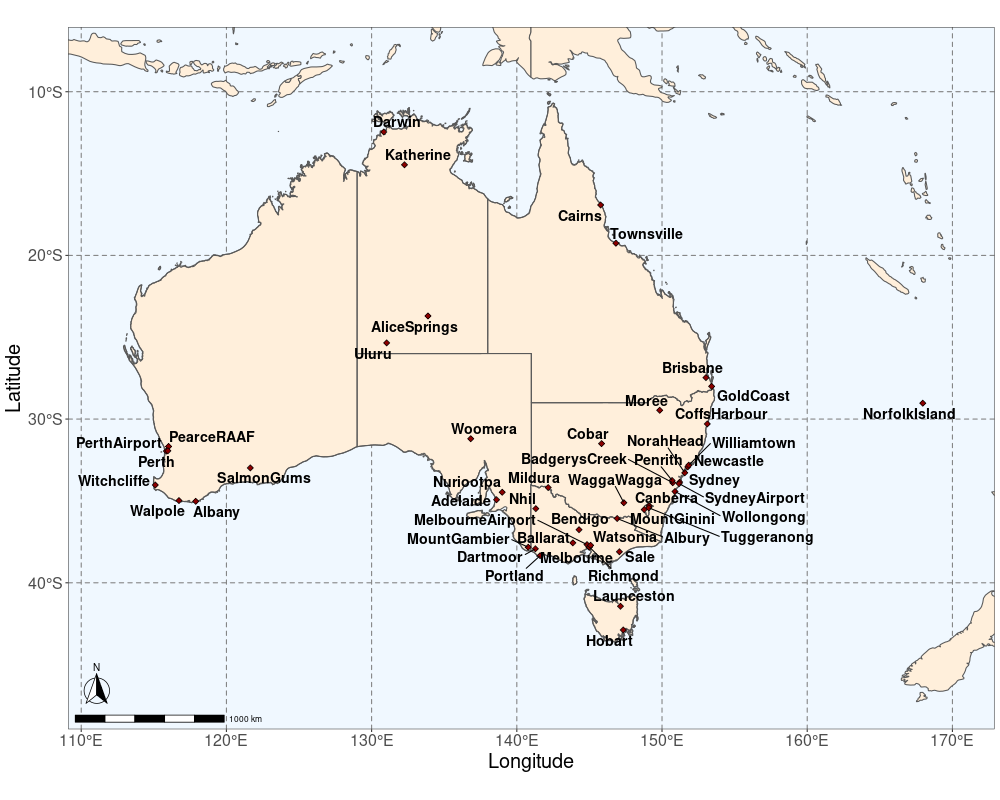
\includegraphics[width=0.7\textwidth]{Images/Cartographie/Australia_full_map.png}
    \caption{Carte de l'Australie et villes dont la météo est observée}
\end{figure}

Nous pouvons desormais utiliser les colonnes de longitude et latitude à la place de la colonne localisation. 

\section{Etude des climats}

Maintenant que nous pouvons afficher les lieux sur une carte, nous pouvons déterminer à quelle zone climatique appartient chaque point.

Comme on peut le voir sur la carte précédente, la plupart des observations ont lieu dans le sud-est du pays, où la concentration d'habitants et de ville est la plus grande. Cette zone correspond à un climat tempéré pour les villes les plus au sud et subtropical pour les villes plus au nord comme Brisbane. Au nord du pays nous avons les villes sur les littoraux dans une zone plus tropicale, et enfin au sud-ouest nous avons d'autre villes subtropicales. Plus à l'intérieur des terres, où il le climat est désertique, nous avons les observations de Uluru, Alice Springs et Woomera. Enfin, nous avons aussi les données de villes sur l'île de Tasmanie et l'île Norfolk. 

\begin{figure}[H]
    \centering
    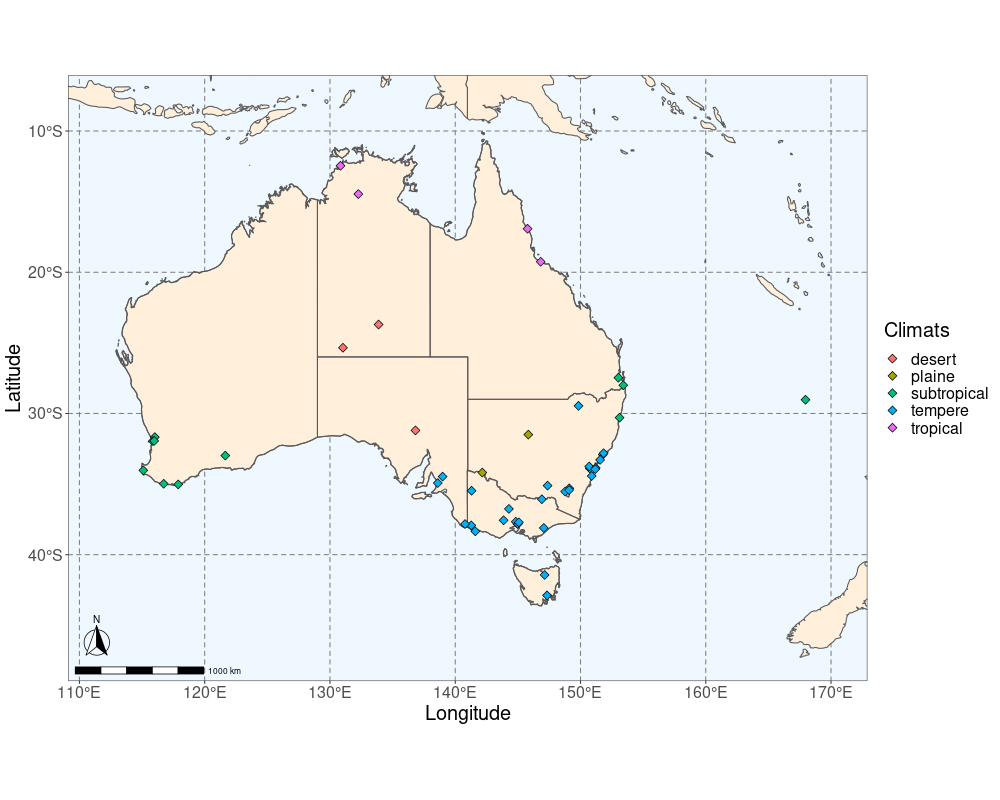
\includegraphics[width=0.7\textwidth]{Images/Cartographie/Australia_climates.png}
    \caption{Carte de l'Australie et climat des villes}
\end{figure}

Nous avons donc les observations de 4 lieux tropicaux, 3 lieux désertiques, 2 lieux dans les plaines (le climat de transition entre désertique et tempéré, en quelques sortes), 11 lieux subtropicaux et enfin 29 lieux tempérés. Certaines données sont liées à des villes mais d'autres à des aéroport ou encore des lieux touristiques.

\subsection{Particularités des climats et périodicité}

Les données étant étalées sur 10 ans, on peut trouver une périodicité dans les mesures à l'année. Nous pouvons alors, pour chaque ville, faire un graphique comprenant les moyennes des température maximales, minimales et moyennes de chaque jour sur 10 ans. Et faire de même pour les précipitations. 

Nous pouvons afficher ces données en fonction des saisons. Nous pourrons ainsi remplacer la variable date par une variable avec uniquement 4 niveaux différents comme expliqué précédemment, à savoir les saisons. Nous prendrons comme saisons : 

\begin{itemize}
    \item L’été, de décembre à février
    \item L’automne, de mars à mai
    \item L’hiver, de juin à août
    \item Le printemps, de septembre à novembre
\end{itemize}

Nous obtenons les graphiques de la Figure \ref{fig:temp_and_rainfall}

\begin{figure}[p]
    \centering
        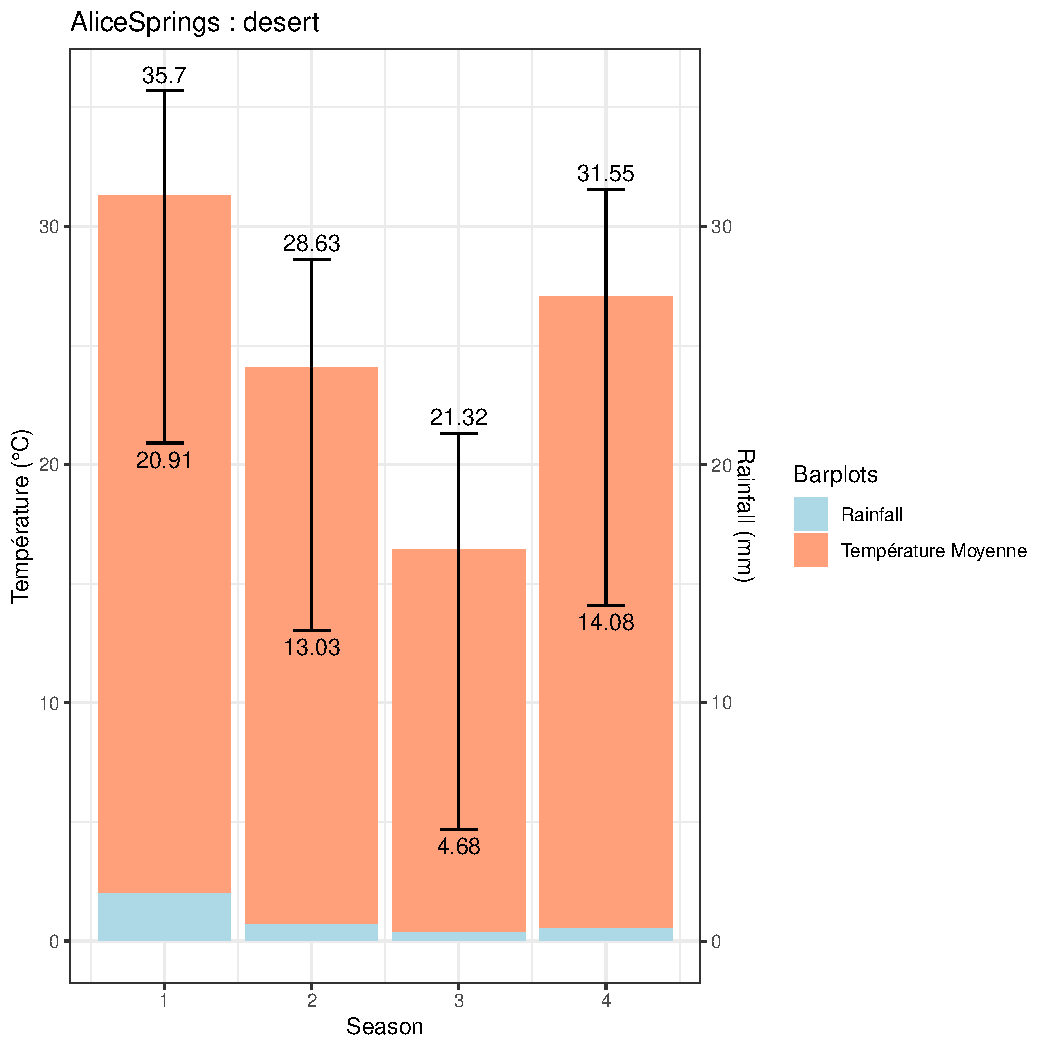
\includegraphics[page=1,width=0.4\textwidth]{Images/Temp_and_Rainfalldesert.pdf}
        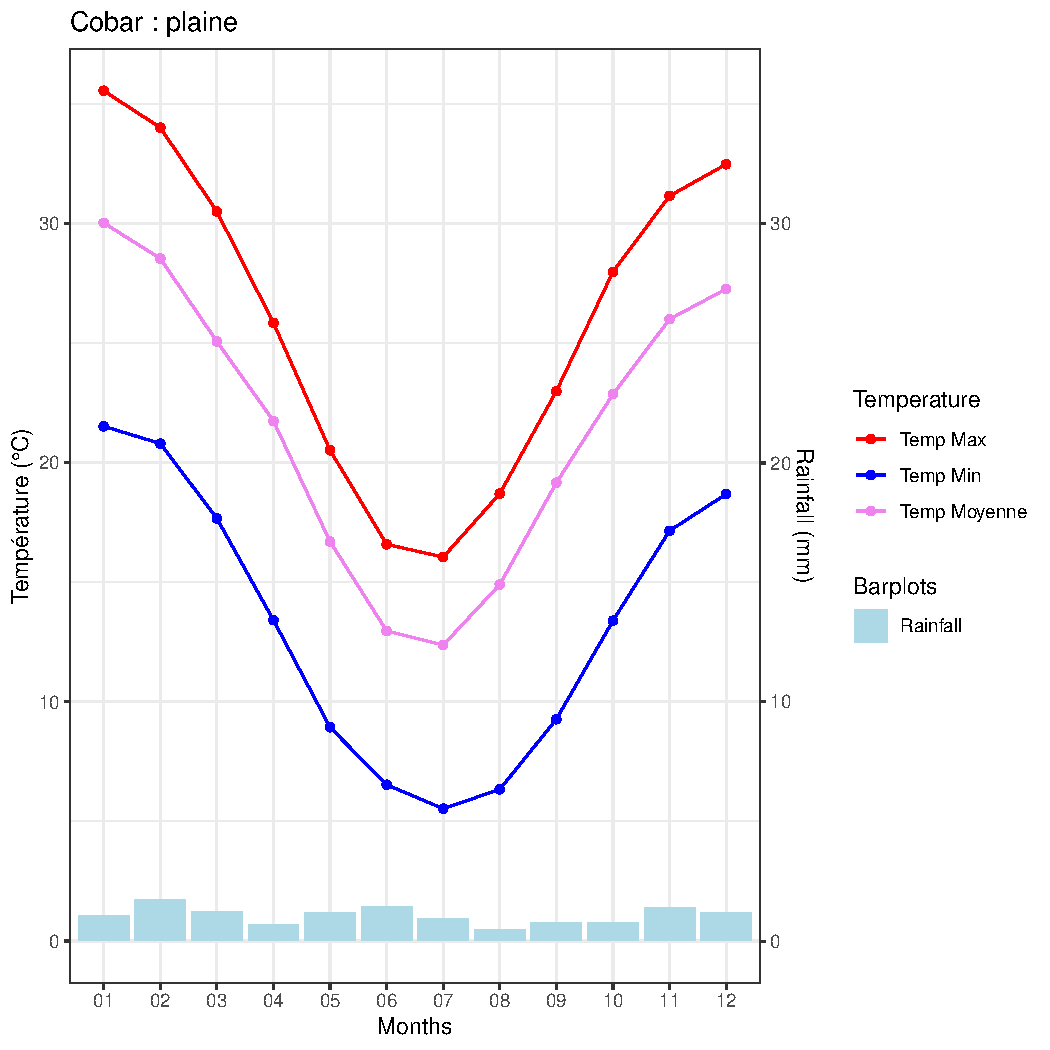
\includegraphics[page=1,width=0.4\textwidth]{Images/Temp_and_Rainfallplaine.pdf}
        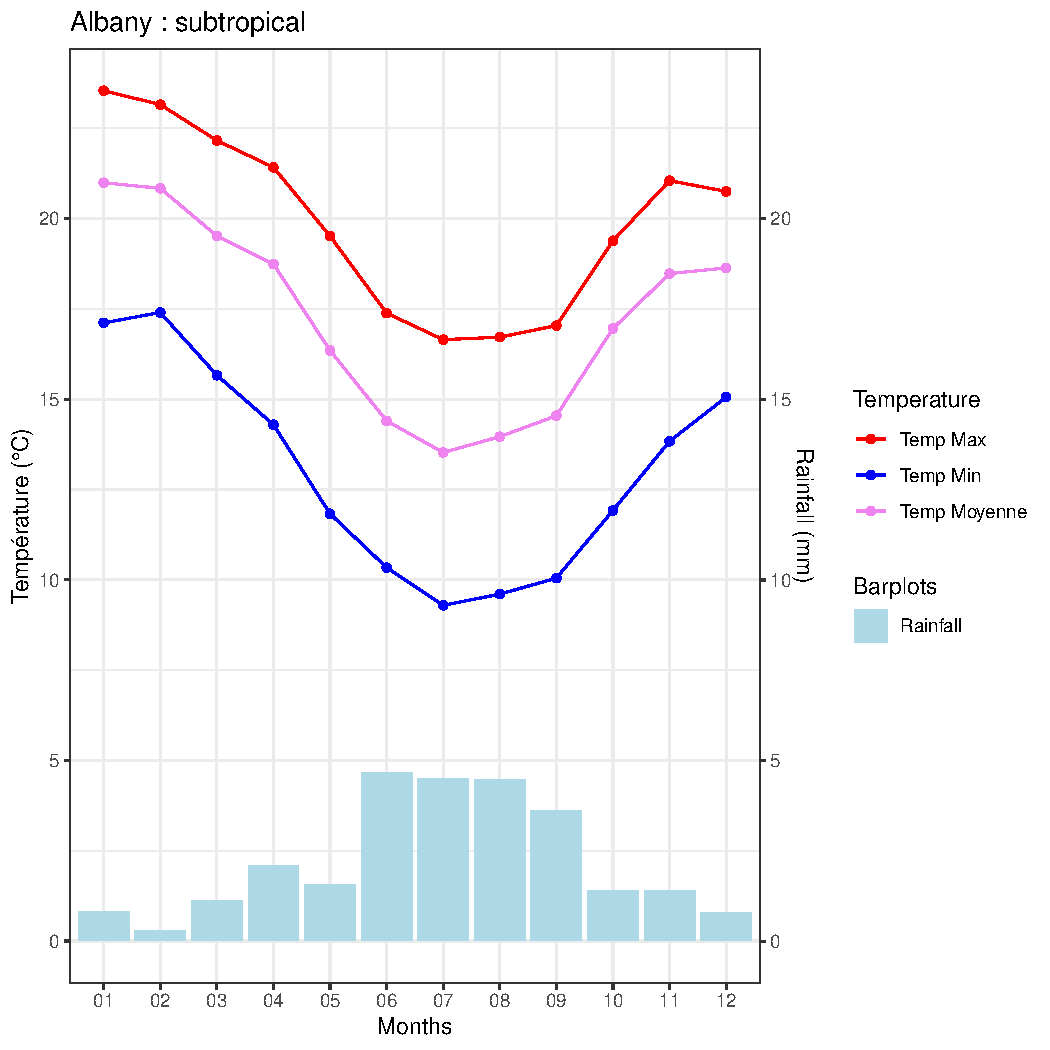
\includegraphics[page=1,width=0.4\textwidth]{Images/Temp_and_Rainfallsubtropical.pdf}
        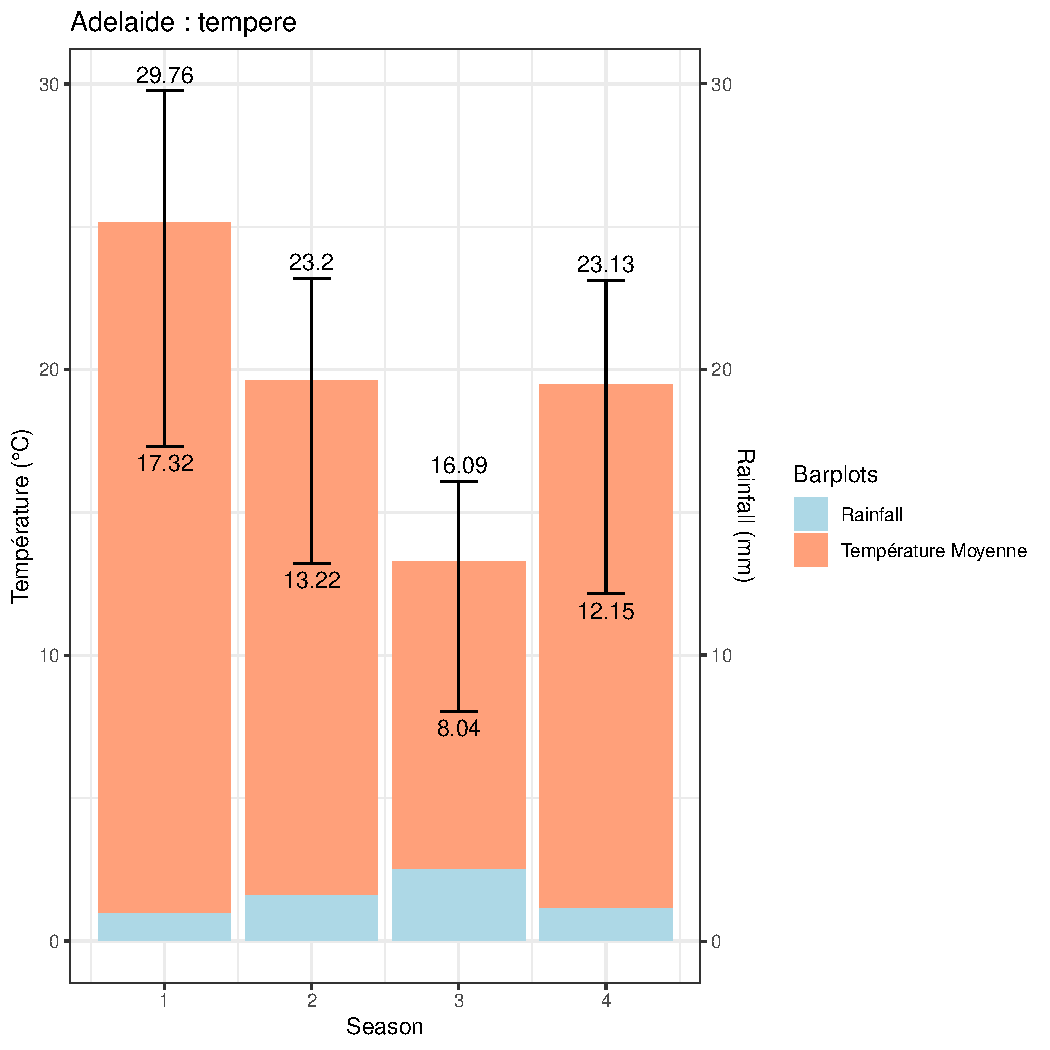
\includegraphics[page=1,width=0.4\textwidth]{Images/Temp_and_Rainfalltempere.pdf}
        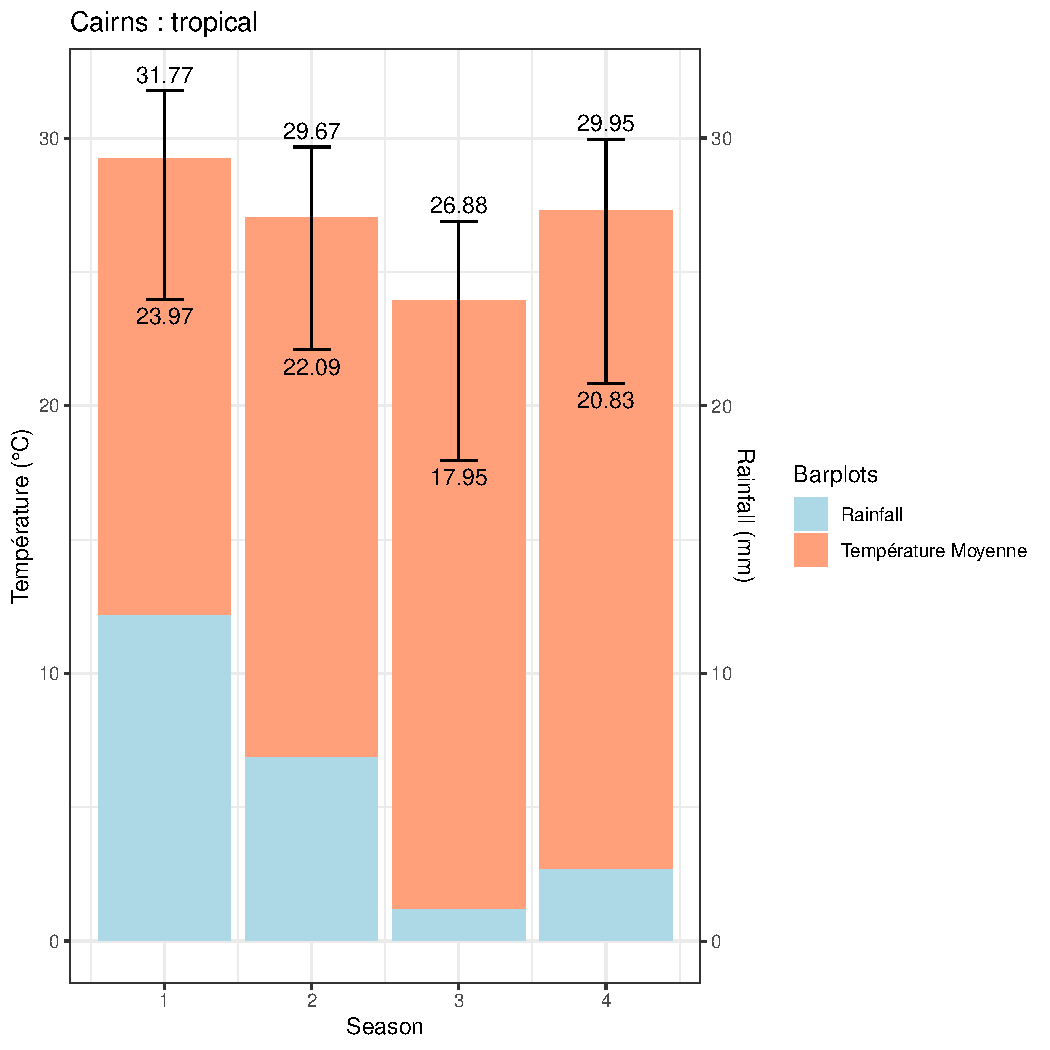
\includegraphics[page=1,width=0.4\textwidth]{Images/Temp_and_Rainfalltropical.pdf}
    \caption{Température Minimale et Maximale ainsi que pluviométrie au cours d'une année pour certaines des villes des données (une par climat)}
    \label{fig:temp_and_rainfall}
\end{figure}

On remarque tout de suite que les températures les plus élevées sont aux alentours de décembre / janvier; l'Australie étant dans l'hémisphère Sud, il s'agit de l'été. 

On remarque ensuite quelques particularité dues aux climats. Dans les régions tempérée et subtropicale tout d'abord, nous avons des températures qui évoluent entre en dessous de 10 degrés et environ 30 degrés, avec en hiver (mai, juin, juillet) plus de pluie que sur le reste de l'année.

Du côté des régions dans les plaines, il pleut moins tout au long de l'année et nous n'observons pas de période de pluie comme pour les deux premières régions. Les températures sont en revanche à peu près les même, voire plus chaudes pendant l'été. Lorsque l'on se penche sur les régions désertiques, les températures sont encore plus hautes et les précipitations sont encore moins importantes, avec seulement quelques millimètres tout au long de l'année. 

A l'opposé, dans les régions tropicales, la température tout au long de l'année évolue moins et reste plus proche de 30 degrés tout au long de l'année (avec une légère baisse en hiver). Dans ces régions, il pleut énormément pendant l'hiver et quasiment pas pendant l'été.

Le choix de ne garder que les saisons et pas les dates se justifie par le fait que si nous voulons prédire s'il pleut le lendemain, nous n'avons pas besoin de savoir précisemment quel jour nous sommes, voire quel mois. On remarque sur les graphiques des différences notables entre les saisons, et celle-ci suffiront sûrement pour nous aider à prédire ce que nous voulons. De plus, nous nous débarassons d'une variable avec beaucoup de facteurs différents, ce qui nous sera bénéfique lors de la mise en place de modèle de prédictions.

Nous nous retrouvons au final avec les variables suivantes : 
\begin{itemize}
    \item MinTemp, MaxTemp, Temp9am, Temp3pm
    \item Rainfall, RainToday, RainTomorrow, Evaporation
    \item Sunshine, Cloud9am, Cloud3pm
    \item WindGustDir, WindGustSpeed, WindDir9am, WindDir3pm, WindSpeed9am, WindSpeed3pm
    \item Humidity9am, Humidity3pm
    \item Pressure9am, Pressure3pm
    \item Season, Climate
    \item Latitude, Longitude
\end{itemize}
Qui sont toutes des variables numériques (0 ou 1 pour les variables booléennes RainToday et RainTomorrow).

\section{Complétion des données}

\subsection{Pourquoi compléter ?}

Afin de se rendre compte de la distribution des valeurs manquantes, on affiche ce qu'on appelle la missingness map de nos données (Figure \ref{fig:missingness_raw}).

\begin{figure}[ht]
    \centering
    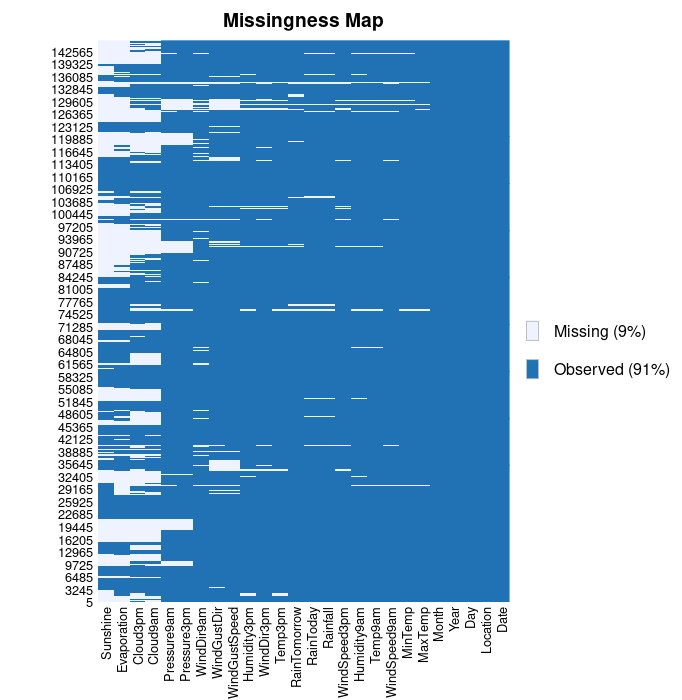
\includegraphics[width=0.5\textwidth]{Images/missmap.png}
    \caption{Missingness Map des données avant la complétion.}
    \label{fig:missingness_raw}
\end{figure}

Afin de faire des prédictions sur nos données, nous avons besoin de nous débarasser des observations avec des valeurs \emph{NA}. Pour cela, on utilise la commande \mintinline{R}{na.omit}. On se retrouve avec $56420$ observations sur les $145460$ de base, ce qui est très peu. De plus, la plupart des lieux ne sont plus représentés comme nous l'indique la Figure \ref{fig:distrib_raw}.

\begin{figure}[H]
    \centering
    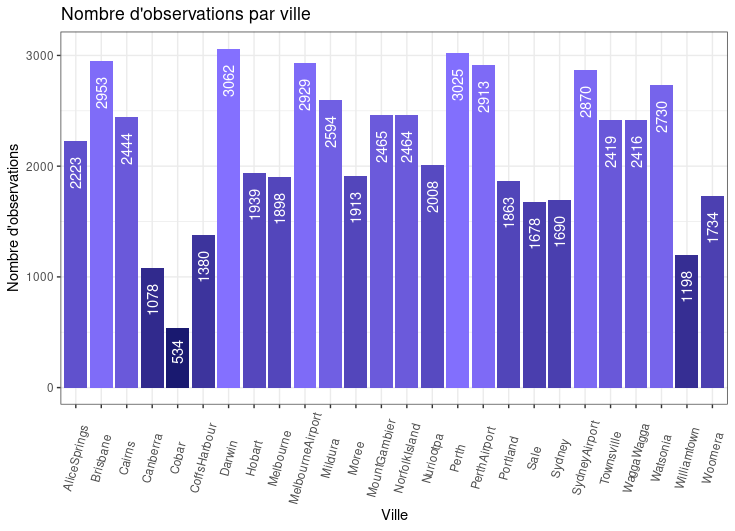
\includegraphics[width=0.6\textwidth]{Images/distribution_lieux_raw.png}
    \caption{Distribution du nombre d'observations après un \emph{na.omit}.}
    \label{fig:distrib_raw}
\end{figure}

Nous allons donc chercher un moyen de compléter les valeurs \emph{NA}, et de le faire de façon à ne pas avoir trop de données redondantes et de garder une cohérence vis-à-vis des climats : nous allons copier les données d'un lieu à l'autre d'une certaine façon.

\subsection{Comment compléter ?}

Pour compléter nos données, nous allons regarder pour chaque variable quels sont les lieux qui ont besoin de complétion, disons ceux qui ont plus de 20\% de \emph{NA} pour cette variable, et quels sont ceux avec lesquels nous pouvons compléter : les autres qui ont plus de 2500 observations et qui ont au moins 80\% de leurs observations complètes. Nous excluons ainsi les lieux dont nous n'avons pas les observations sur les dix années : lorsque nous complétons nos données, nous voulons que les dates coincident pour ne pas perdre en cohérence, ainsi nous voulons compléter les données avec les lieux pour lesquels nous avons des observation sur la période maximale d'observation de notre base de données, soit plus de 2500 jours. Le seuil de 80\% des données est choisi pour avoir un maximum d'observations sans \emph{NA} et pour être sûr d'avoir une ville depuis laquelle copier les données.

Lorsque nous copions les données d'un lieu à un autre, nous nous soucions donc de la date d'observation. Cependant, cela ne suffira pas. Nous avons vu en effet que les différents lieux observés appartiennet à des zones climatiques très différentes. Pour chaque variable, nous allons donc associer nos deux listes de lieux (ceux à compléter et ceux avec lesquels compléter) en cherchant les lieux les plus proches de la même zone climatique.

Au final, nous nous retrouvons avec une liste de couples pour chaque variable.

Avec cette méthode, nous allons copier jusqu'à 5 fois maximum les données d'un lieu pour un autre lieu, et nous le ferons de manière "intelligente", sans perte de cohérence par rapport aux climats des lieux observés. Nous pouvons afficher quelles données de quelles villes vont compléter quelle autre villes sur des cartes comme celle de la Figure \ref{fig:path_data}. On peut voir que pour les variables où il y avait le plus de \emph{NA}, beaucoup de lieux sont complétés. Dans d'autre cas moins extrêmes, nous n'avons copié les données que d'un lieu à un autre. 

\begin{figure}[ht]
    \centering
    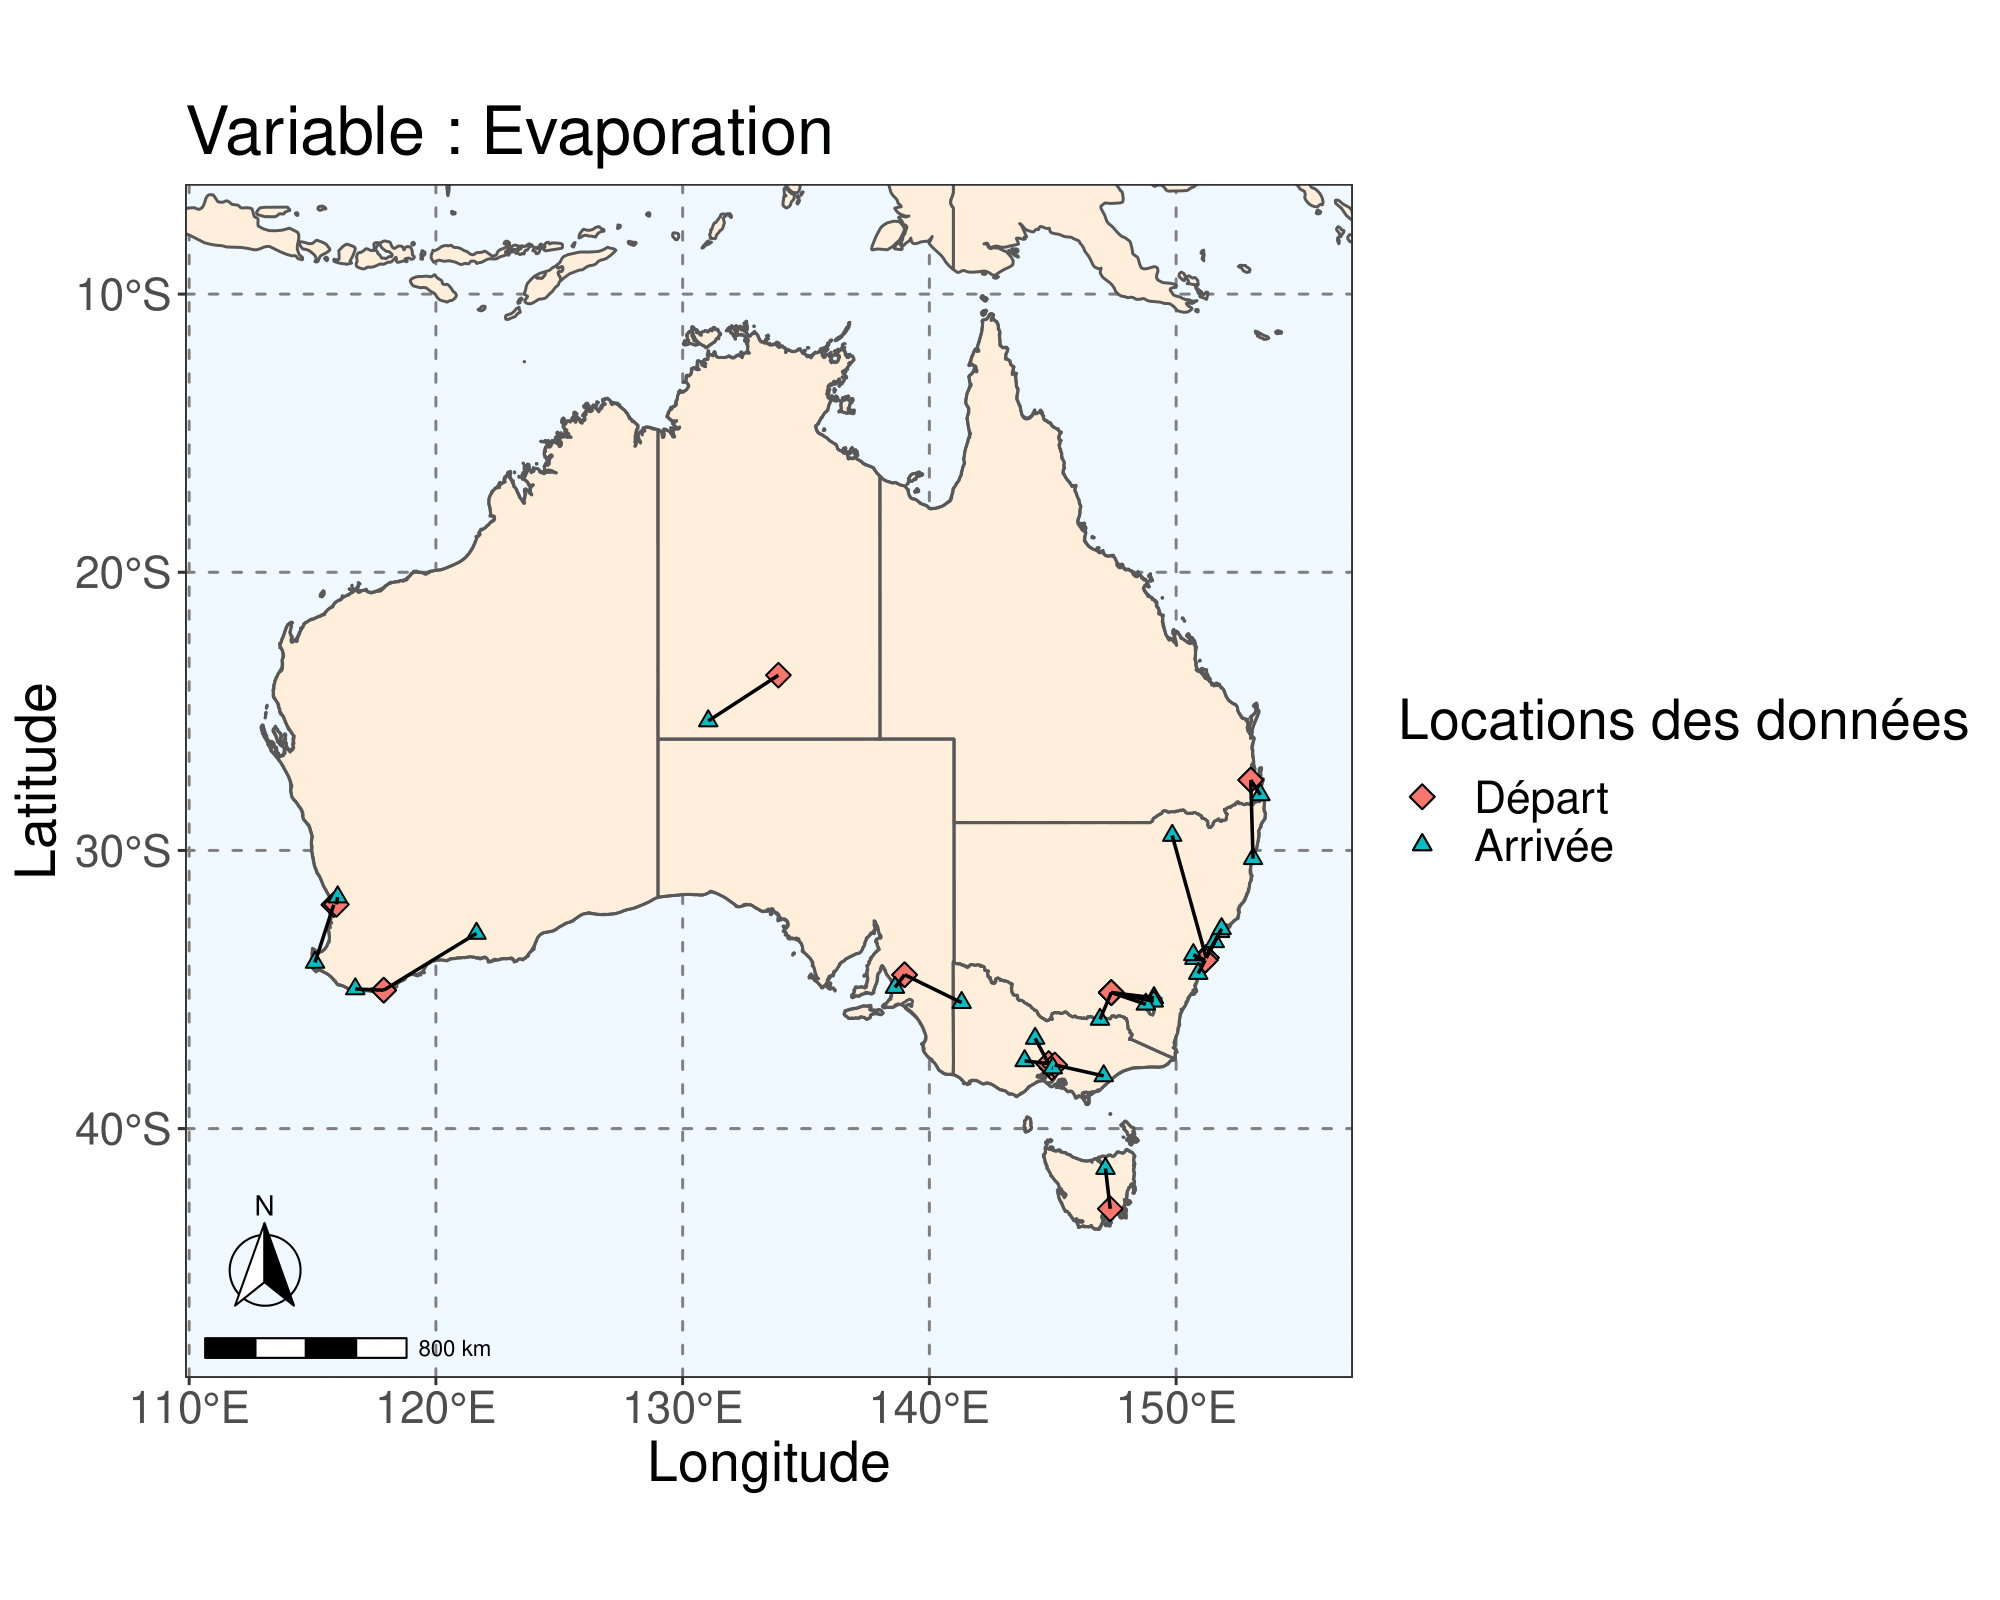
\includegraphics[width=0.45\textwidth]{Images/Australia_map_segments_complete/Australia_map_segments_complete-02.png}
    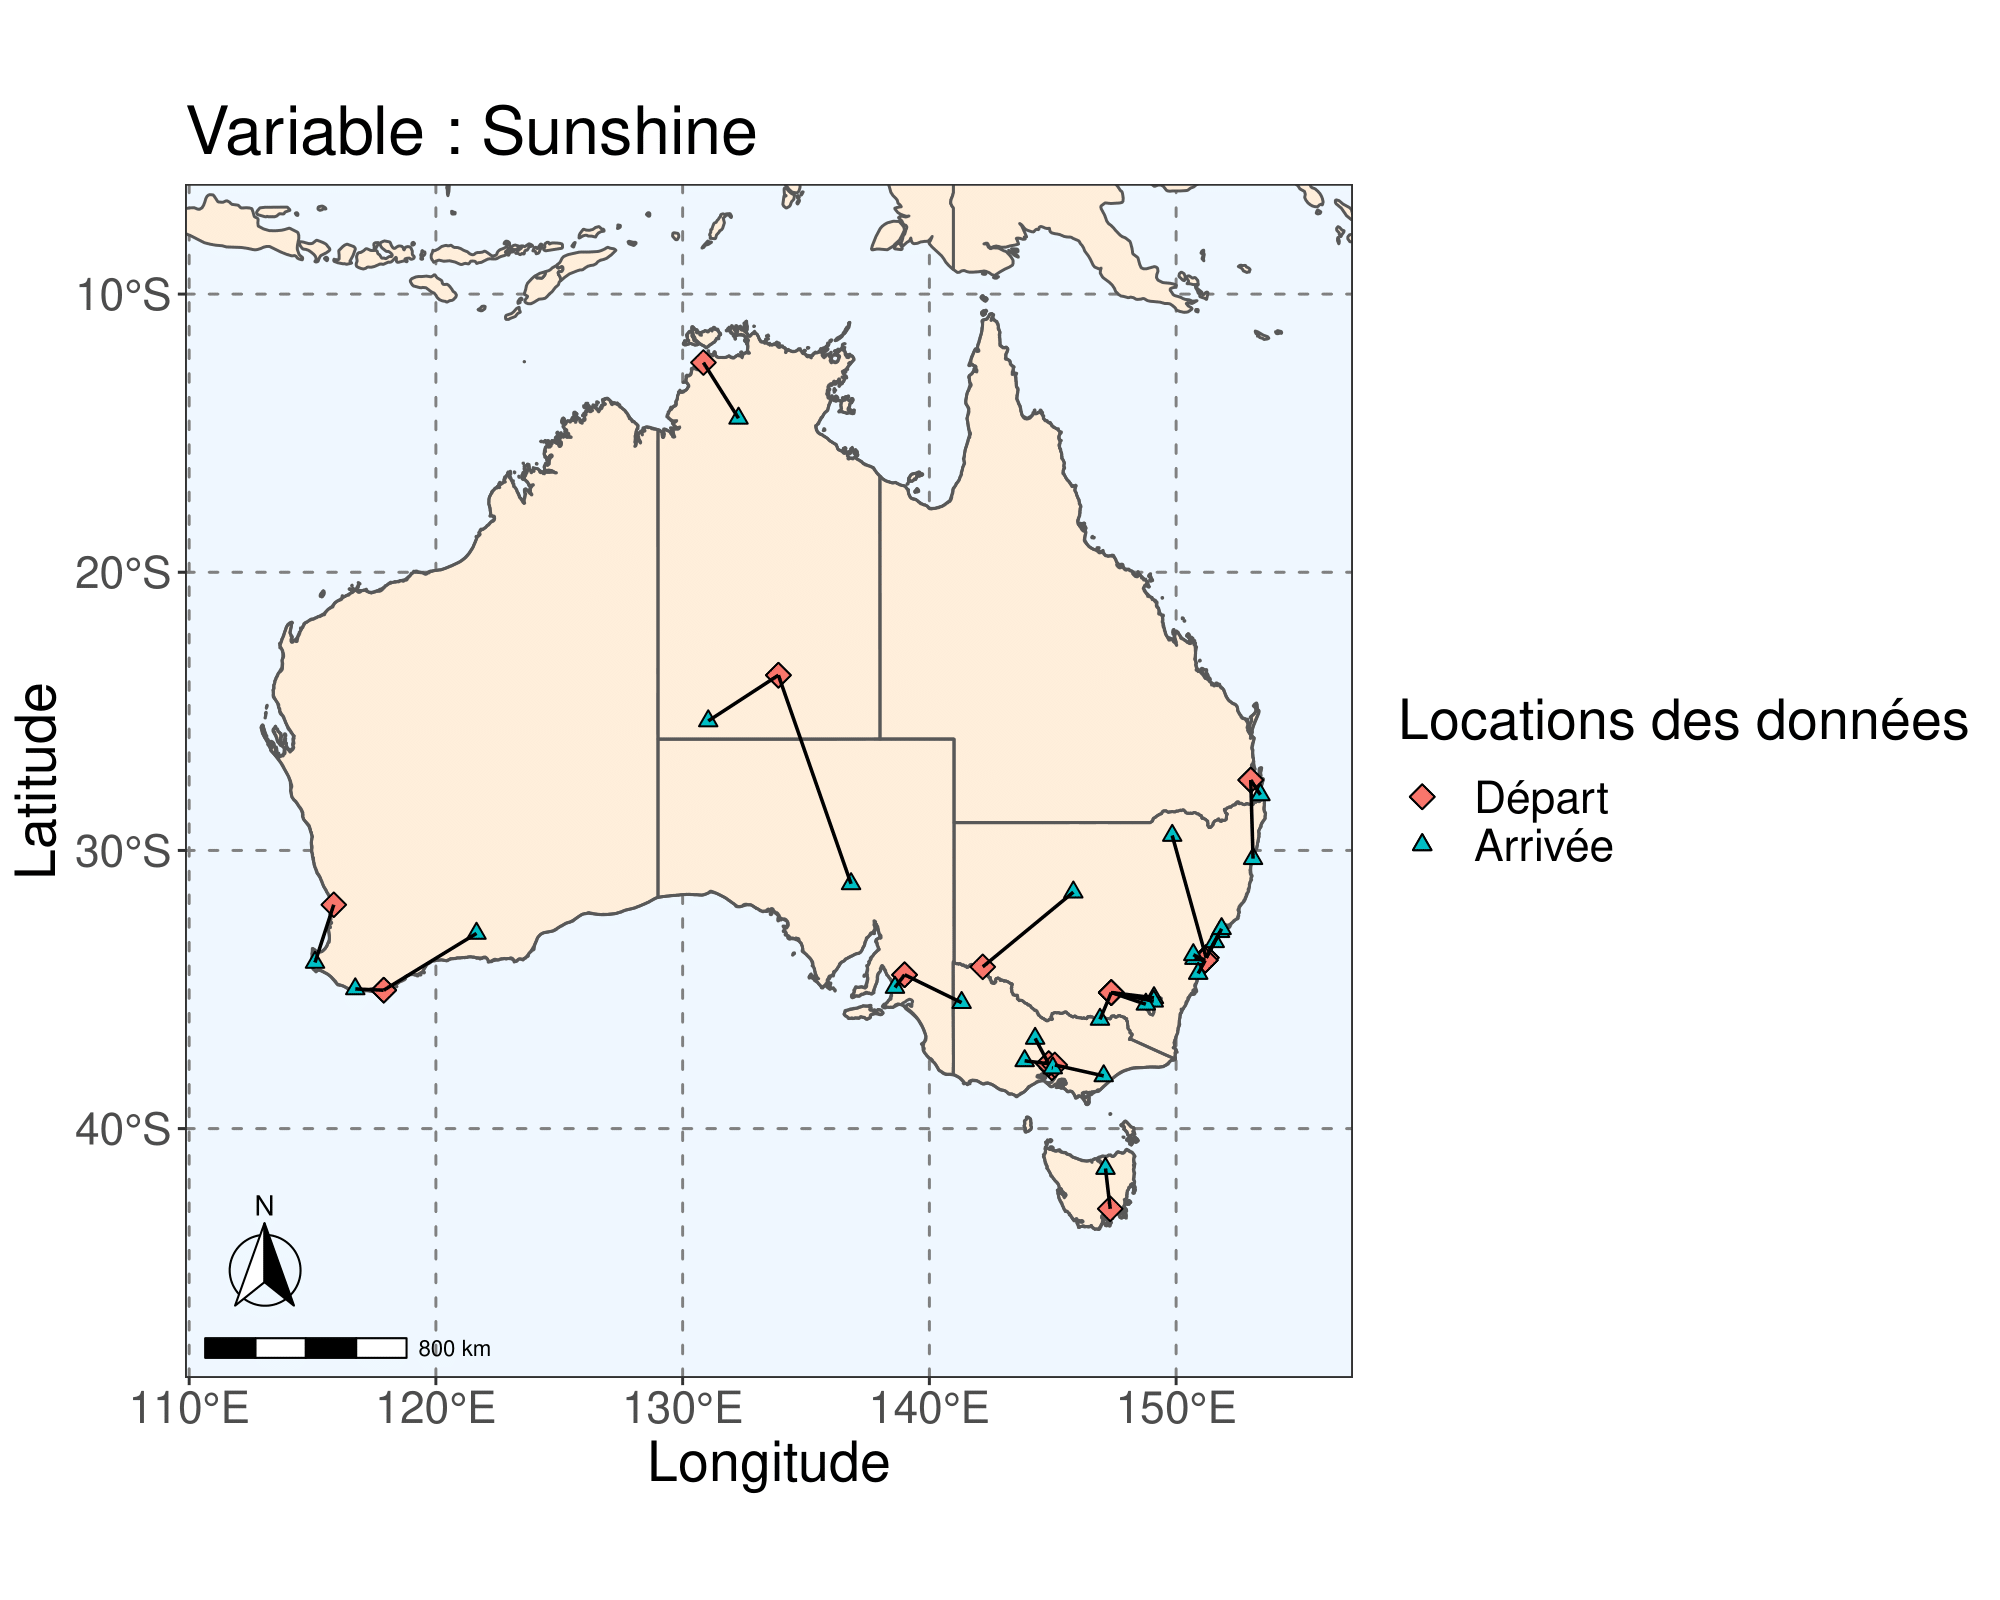
\includegraphics[width=0.45\textwidth]{Images/Australia_map_segments_complete/Australia_map_segments_complete-03.png}
    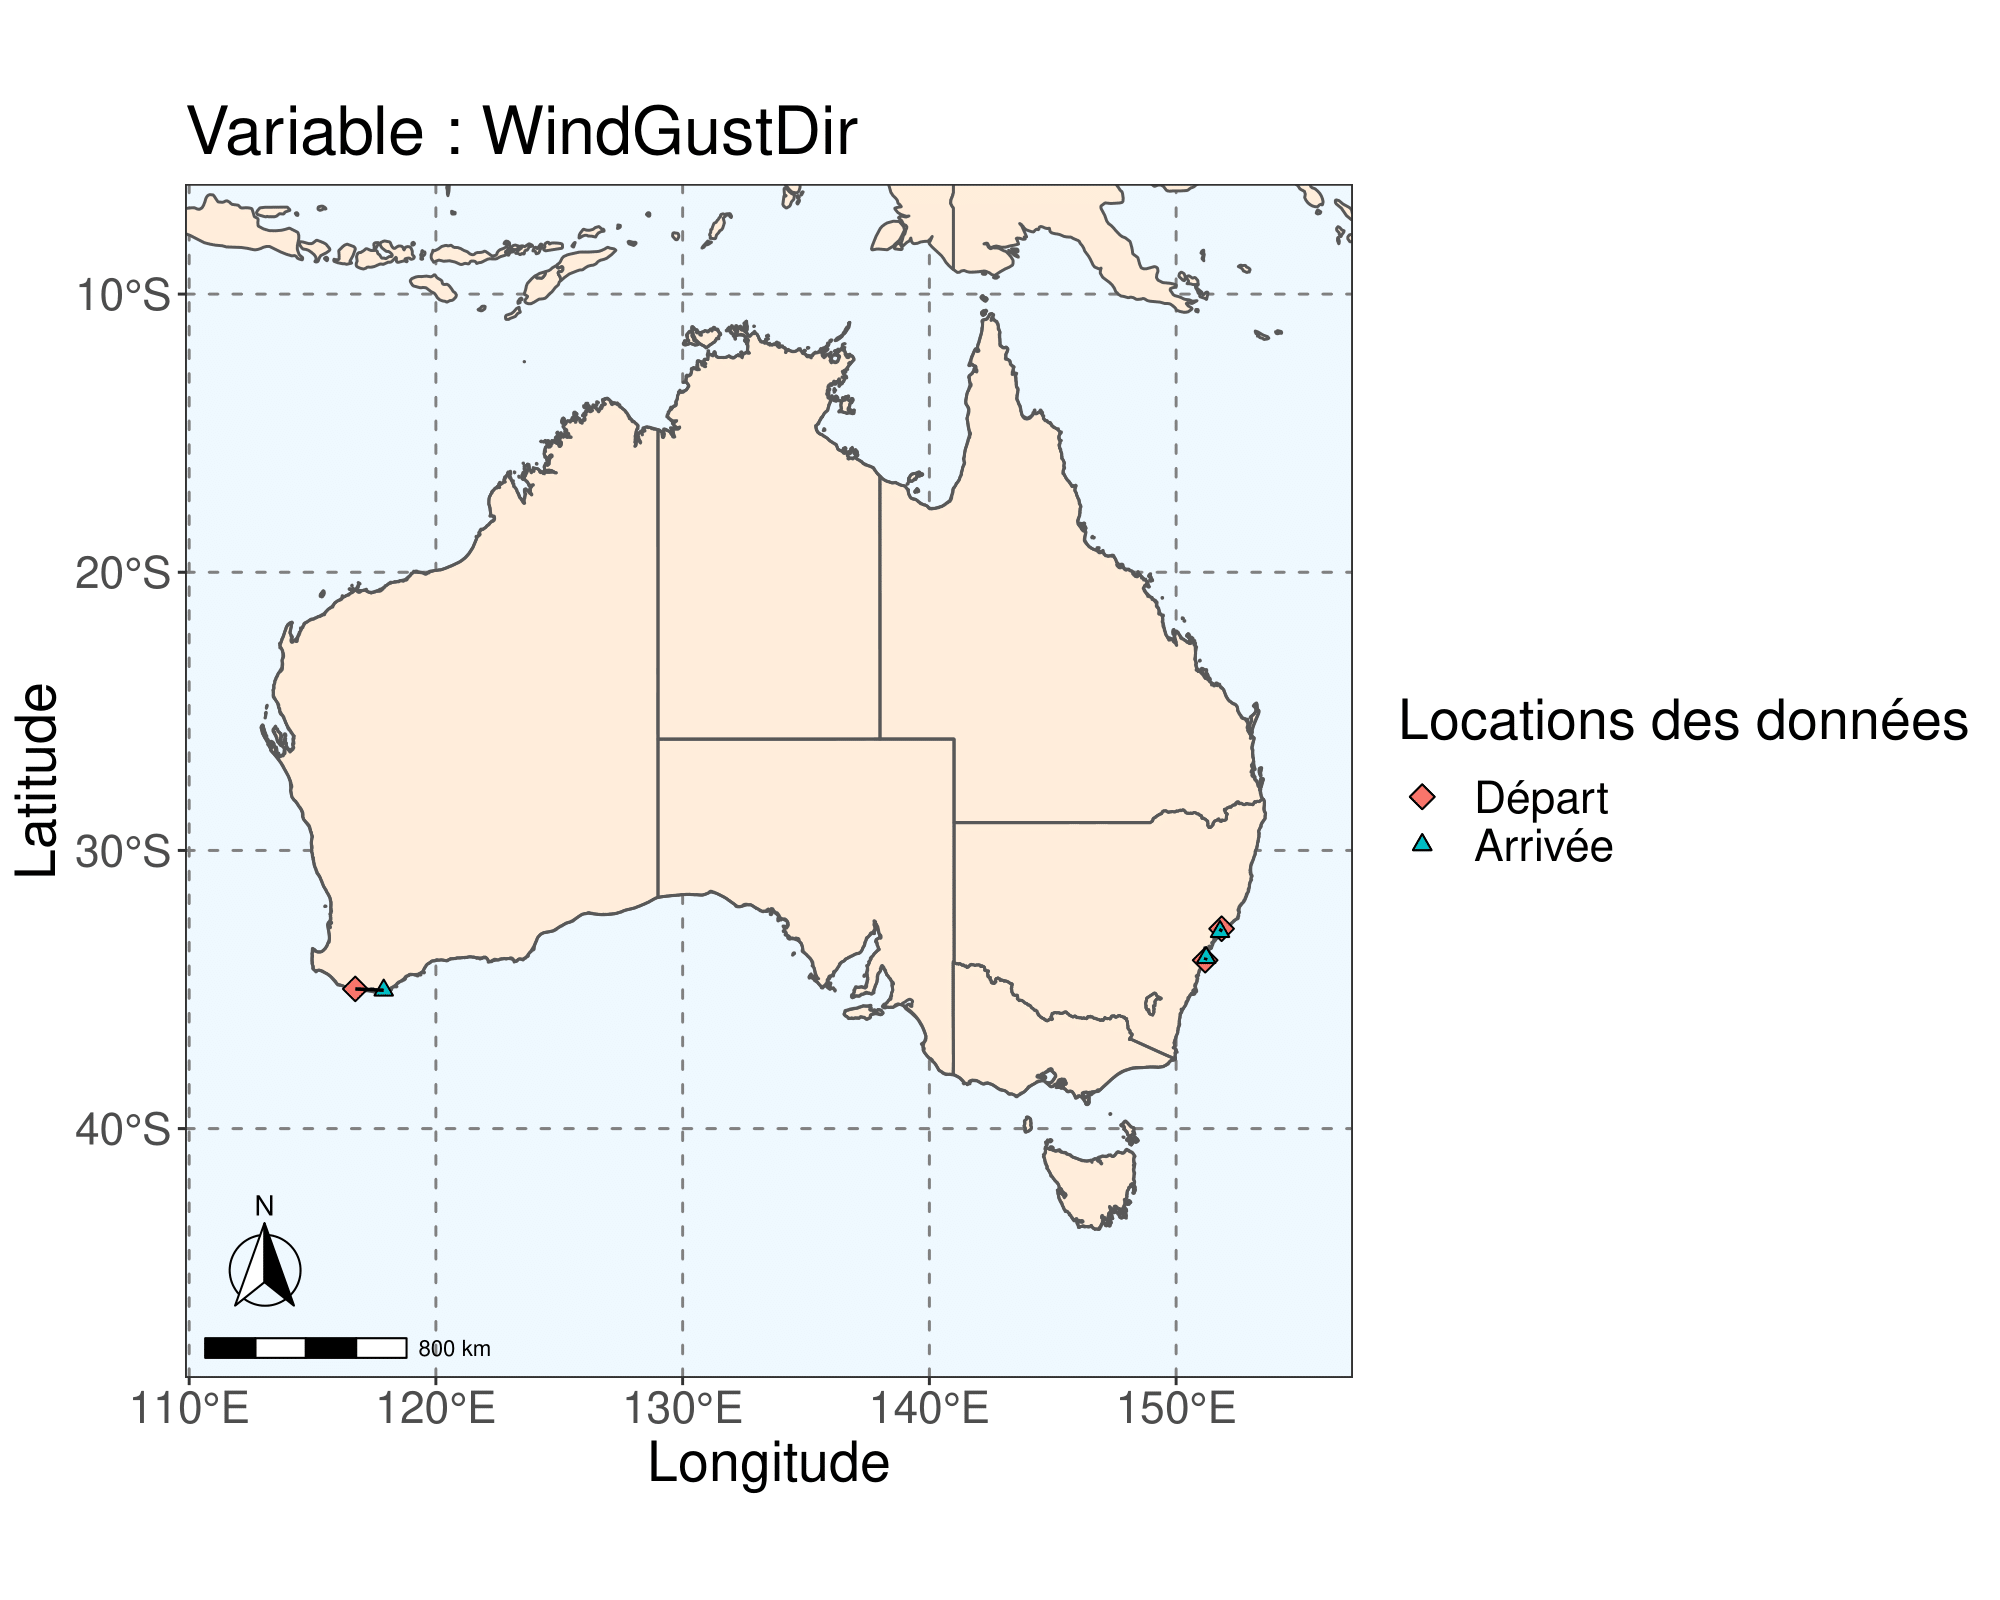
\includegraphics[width=0.45\textwidth]{Images/Australia_map_segments_complete/Australia_map_segments_complete-04.png}
    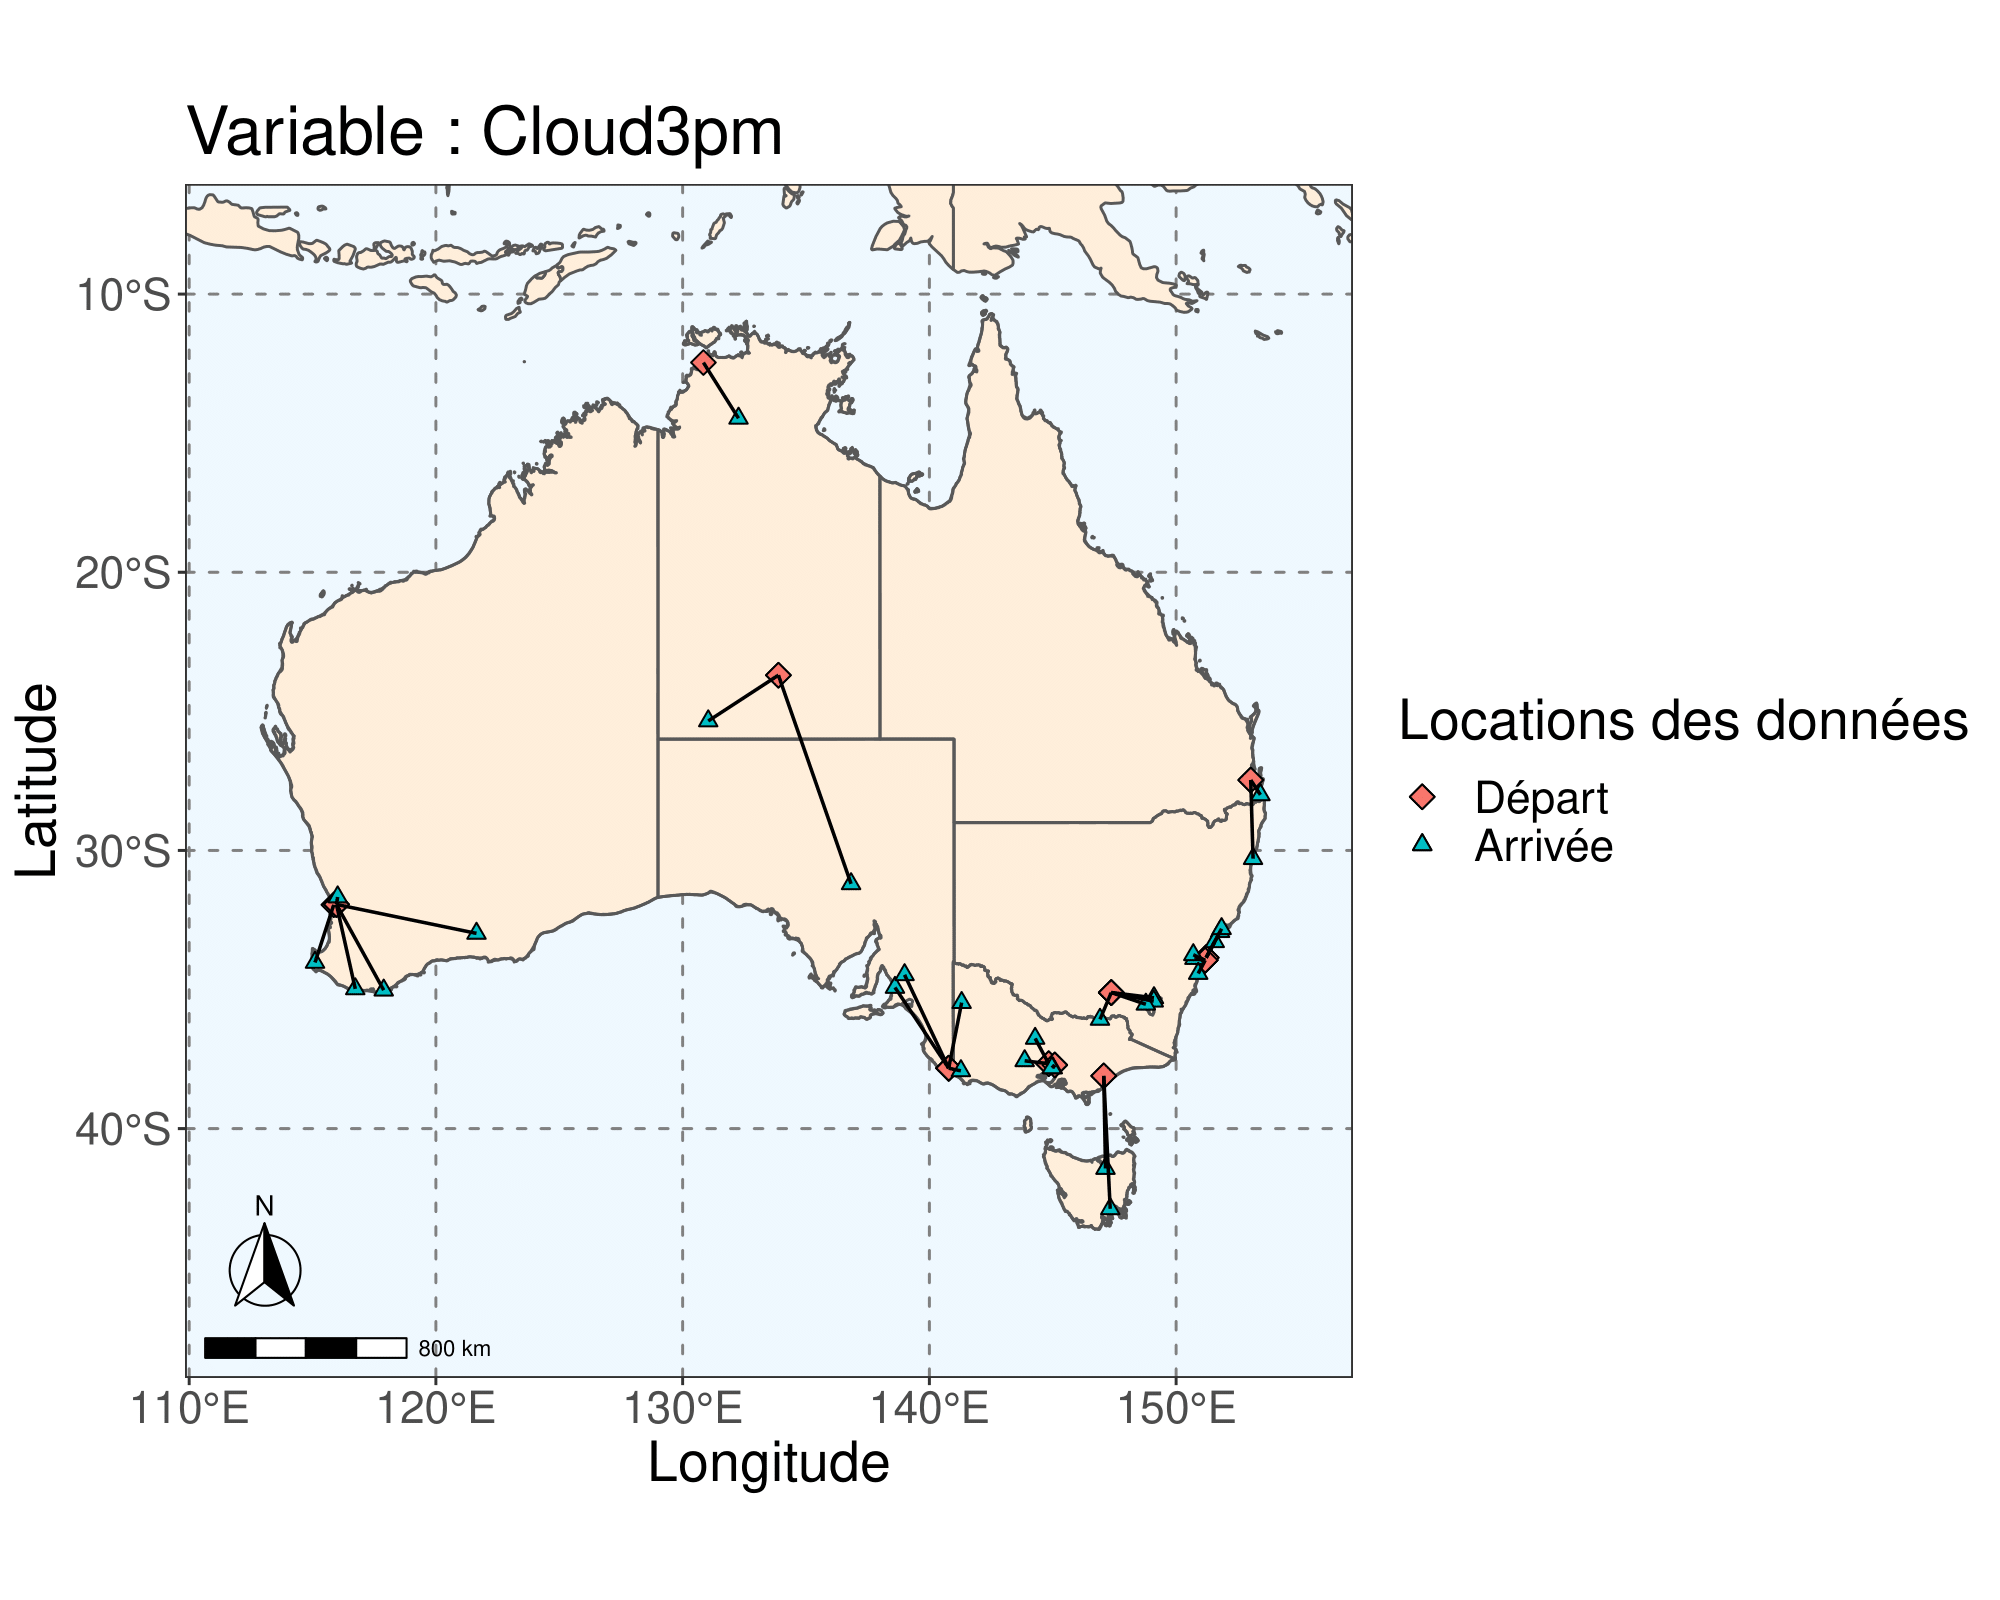
\includegraphics[width=0.45\textwidth]{Images/Australia_map_segments_complete/Australia_map_segments_complete-13.png}
    \caption{Chemin des observations copiées (ville de départ et ville(s) d'arrivée(s)) pour certaines des variables complétées.}
    \label{fig:path_data}
\end{figure}

\subsection{Après complétion}

Au final, le \emph{na.omit} nous donne une base de données avec $105546$ observations. On peut réafficher la missingness map et la distribution des observations par lieu (respectivement Figures \ref{fig:missingness_completed} et \ref{fig:distrib_completed})

\begin{figure}[ht]
    \centering
    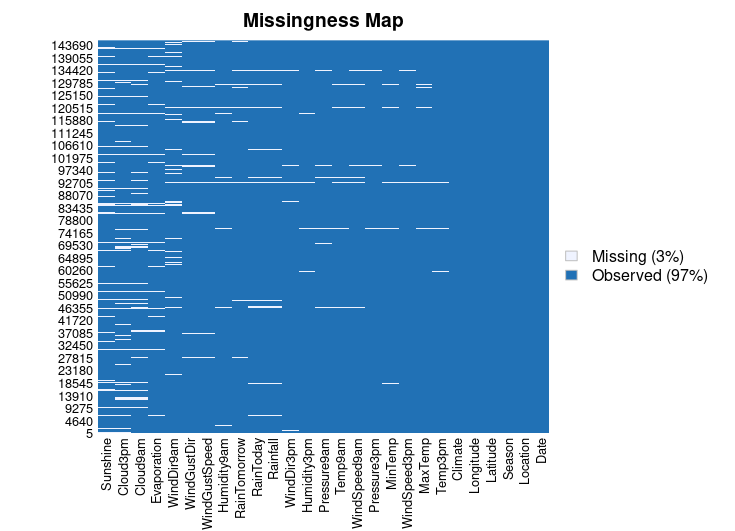
\includegraphics[width=0.5\textwidth]{Images/missmap_completed.png}
    \caption{Missingness Map des données complétées.}
    \label{fig:missingness_completed}
\end{figure}

\begin{figure}[ht]
    \centering
    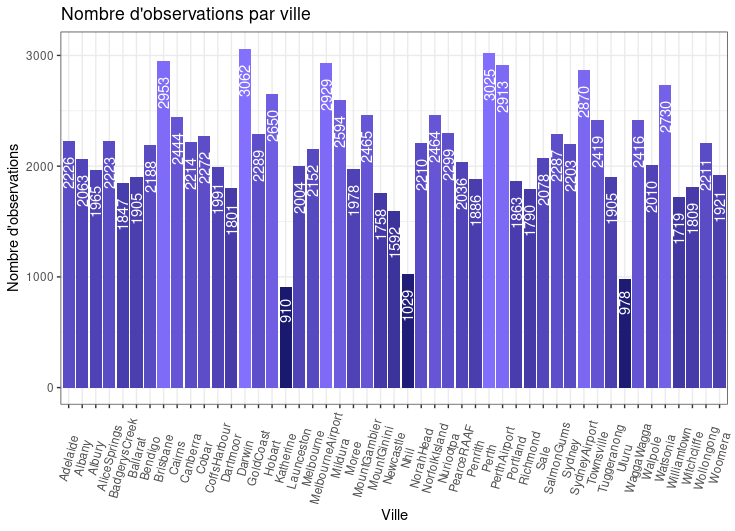
\includegraphics[width=0.6\textwidth]{Images/distribution_lieux_completed.png}
    \caption{Distribution des observations par villes dans notre base de données finale.}
    \label{fig:distrib_completed}
\end{figure}

On remarque que certaines plages de dates n'ont pas été complétées pour certaines variables, il peut y avoir deux raisons à cela : 
\begin{itemize}
    \item Le lieu pour cette variable n'a pas été considéré comme à compléter, malgré quelques valeurs \emph{NA};
    \item Le lieu qui a servi pour la complétion certaines dates en moins que celles du lieu à compléter.
\end{itemize}
Le nombre d'observations de notre base de données finale reste cependant satisfaisante et tous les lieux y sont représentés.

\section{Relations entre les variables}

Dans cette partie nous allons chercher les relations entre les variables.

\subsection{Corrélations entre les variables numériques}

Commençons tout d'abord par nous renseigner sur les corrélations entre les variables numériques (Figure \ref{fig:correlations}). 

\begin{figure}[htp]
    \centering
    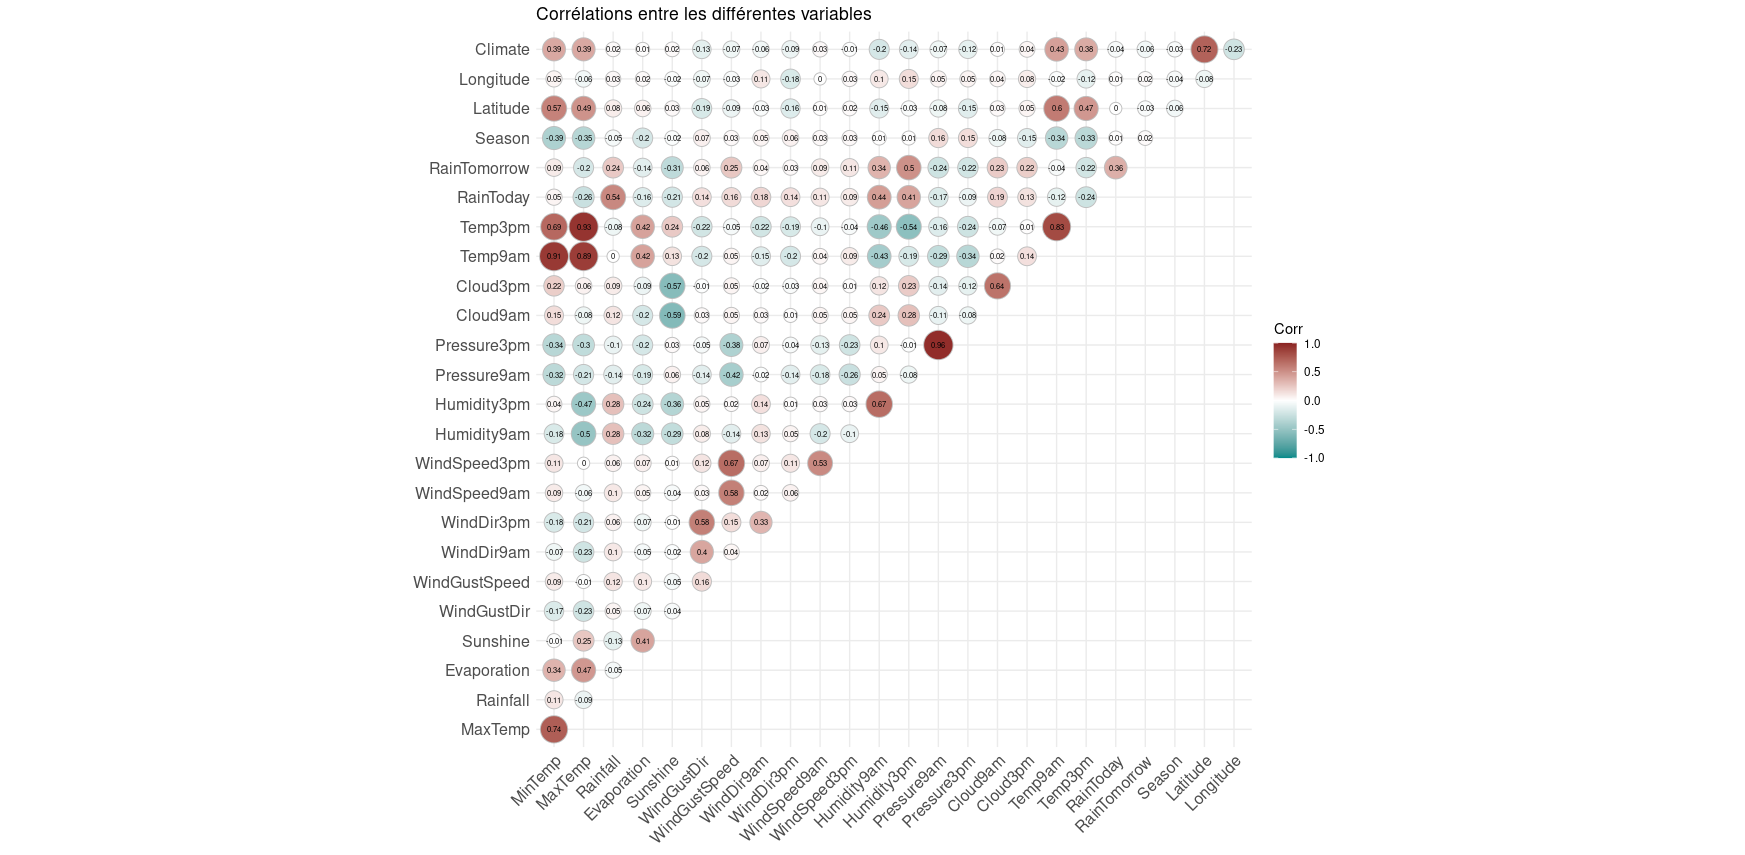
\includegraphics[width=\textwidth]{Images/correlations_variables.png}
    \caption{Corrélations des variables deux-à-deux.}
    \label{fig:correlations}
\end{figure}

Nous pouvons conclure de cette figure les points suivants : 
\begin{itemize}
    \item Concernant les variables de températures : 
    \begin{itemize}
        \item MinTemp et MaxTemp sont deux variables corrélées (coeff. = 0.73). C'est un résultat attendu car ces deux valeurs sont les températures maximales et minimales de la même journée. 
        \item Temp9am et Temp3pm sont fortement corrélées (coeff. = 0.83). Ce résultat était attendu pour la même raison qui explique la corrélation entre MinTemp et MaxTemp.
        \item MinTemp et Temp9am sont très corrélées (coeff. = 0.9). La température minimale d'une journée est atteinte aux alentours de 9h du matin, il est normal d'avoir ce résultat. 
        \item MaxTemp et Temp3pm sont très corrélées (coeff. = 0.94). La température maximale d'une journée est atteinte aux alentours de 15h, ce résultat était donc attendu. 
        \item Nous pouvons aussi remarquer que le couple Temp3pm et MinTemp et le couple Temp9am et MaxTemp sont aussi corrélés (coeff. resp. = 0.69 et 0.89). Comme ces variables sont corrélées entre elles deux à deux, il est normal de trouver ces corrélations. La température maximale est cependant plus corrélées à celle à 9h du matin que ne l'est la température minimale et la température à 15h. Cela peut s'expliquer par le fait qu'en fonction des saisons, le soleil se lève plus ou moins tôt, et que donc à 9h déjà, il peut faire très chaud. Dans tous les cas, il est normal que ces températures soient corrélées puisqu'il s'agit des écarts de températures d'une même journée. Ces derniers ne sont pas très importants et dépendent énormément de la saison (donc de la journée) comme nous l'avons vu Figure \ref{fig:temp_and_rainfall}. 
    \end{itemize}
    \item La variable Latitude est corrélées positivement aux variables de températures (la température dépend des climats et ces climats sont très dépendants de la latitude comme on a pu le voir dans la partie cartographie).
    \item Pression3am et Pression9pm sont très corrélées (coeff. = 0.96) pour les même raisons que les variables de température. Il en va de même pour Humidity3pm et Humidity9am (coeff = 0.66) et WindSpeed3pm et WindSpeed9am (0.49).
    \item WindSpeed3pm est corrélées positivement avec WindGustDir (coeff. = 0.66).
    \item Les variables Cloud9am et Cloud3pm sont corrélées négativement avec la variable Sunshine (-0.57 et -0.55 respectivement) ce qui est logique car ils mesurent à peu près la même chose. 
    \item Les variables d'humidité sont corrélées négativement à MaxTemp (-0.48 et -0.5).
\end{itemize}

\subsection{Boxplots pour les variables à facteurs}

Affichons maintenant les boxplots des valeurs des différents variables continues en fonction de nos variables à facteurs. 

\begin{figure}[htp]
    \centering
    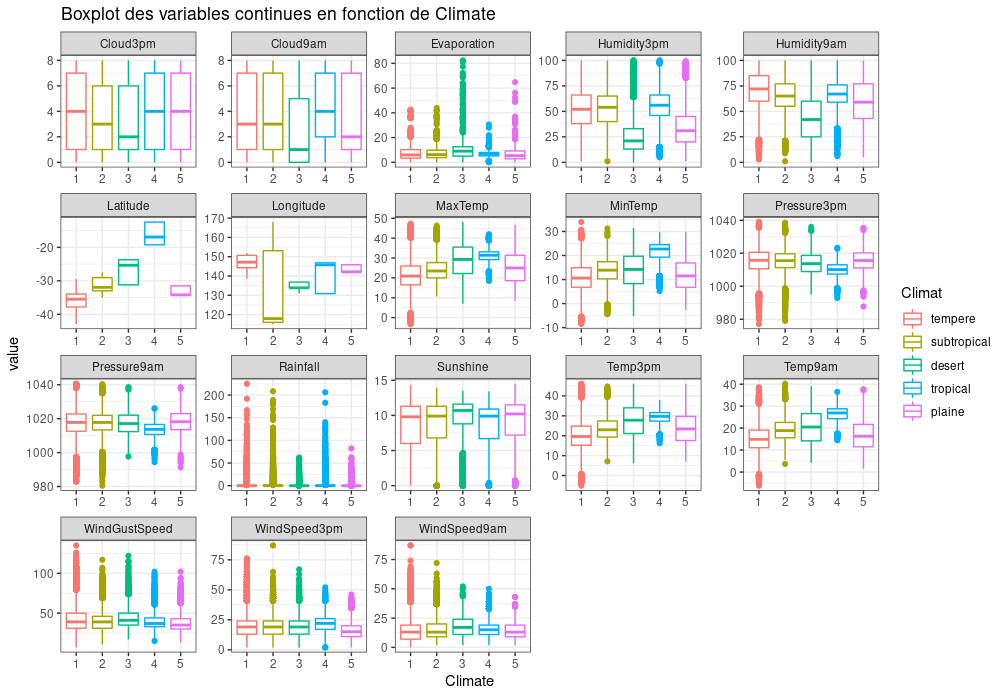
\includegraphics[width=0.8\textwidth]{Images/boxplots/boxplot_Climate.png}
    \caption{Boxplots pour la variable Climate}
    \label{fig:bp_climate}
\end{figure}

Pour la variable Climate (Figure \ref{fig:bp_climate}), on voit une fois de plus la différence entre les climats de désert et de plaine et les autres au niveau de leur humidité, cela se voit aussi avec les grandes valeurs de Rainfall. On peut aussi voir que les climats sont arrangés en couche du nord au sud de l'Australie, comme on pouvait voir sur la carte plus haut. En effet, la région tropicale est au nord du pays, comme l'indique la boîte à moustache concernant la Latitude. Tout au sud on trouve la région tempérée. On peut aussi trouver une différence de températures entre ces 5 climats, avec une distribution ressemblant celle de la Latitude : la région tropicale est la plus chaude, et la moins chauds est la région tempérée. 

\begin{figure}[htp]
    \centering
    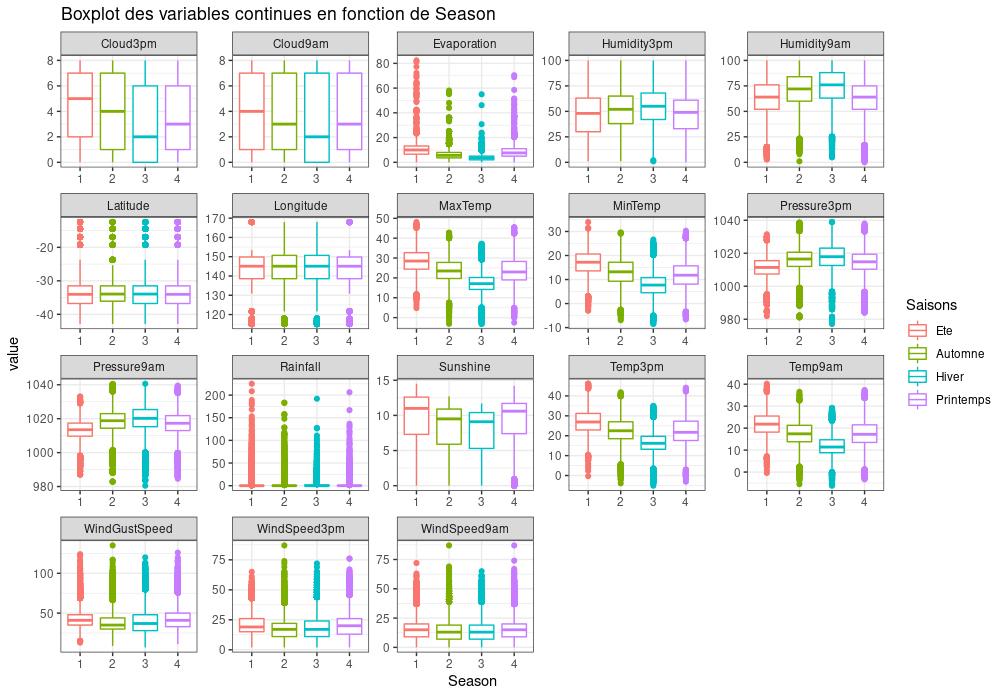
\includegraphics[width=0.8\textwidth]{Images/boxplots/boxplot_Season.png}
    \caption{Boxplots pour la variable Season}
    \label{fig:bp_season}
\end{figure}

Penchons-nous désormais sur les boîtes à moustache de la variable Season (Figure \ref{fig:bp_season}). On trouve la ditribution des températures auxquelles nous nous attendions : il fait plus chaud au été et moins en hiver. Ce même schéma est visible pour le taux d'ensolleillement (et donc un peu pour les variables des nuages). Les variables de pression et d'humidité évolues similairement : elles augmentent en hiver. En effet la pression peut changer en fonction des dépressions (qui apportent souvent le mauvais temps) ou la vitesse du vent \cite{frwiki:190112465}.

\begin{figure}[htp]
    \centering
    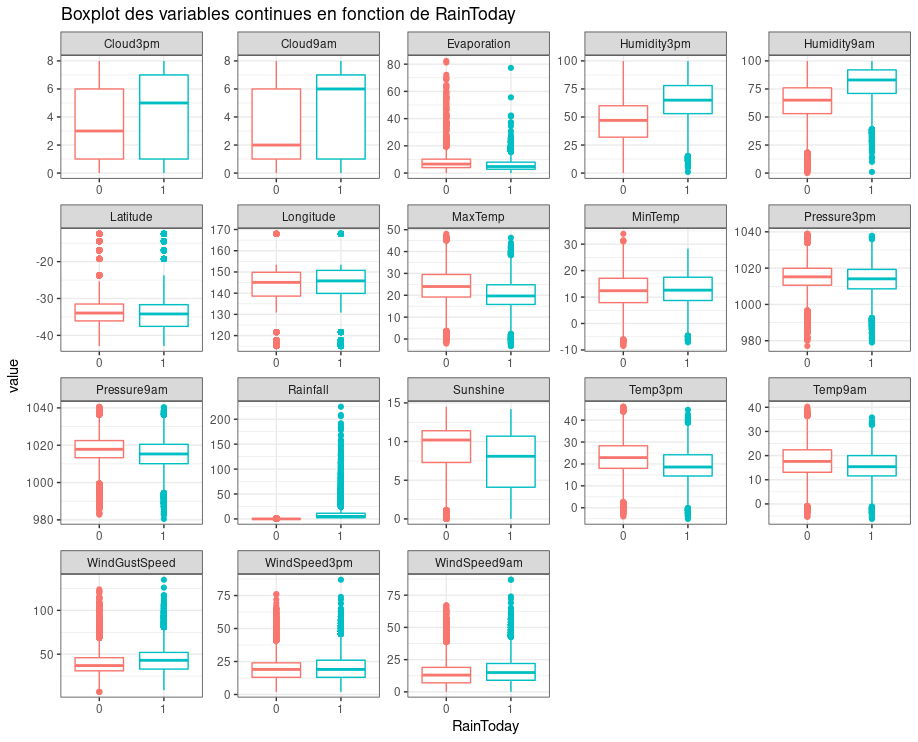
\includegraphics[width=0.7\textwidth]{Images/boxplots/boxplot_RainToday.png}
    \caption{Boxplots pour la variable RainToday}
    \label{fig:bp_raintoday}
\end{figure}

\begin{figure}[htp]
    \centering
    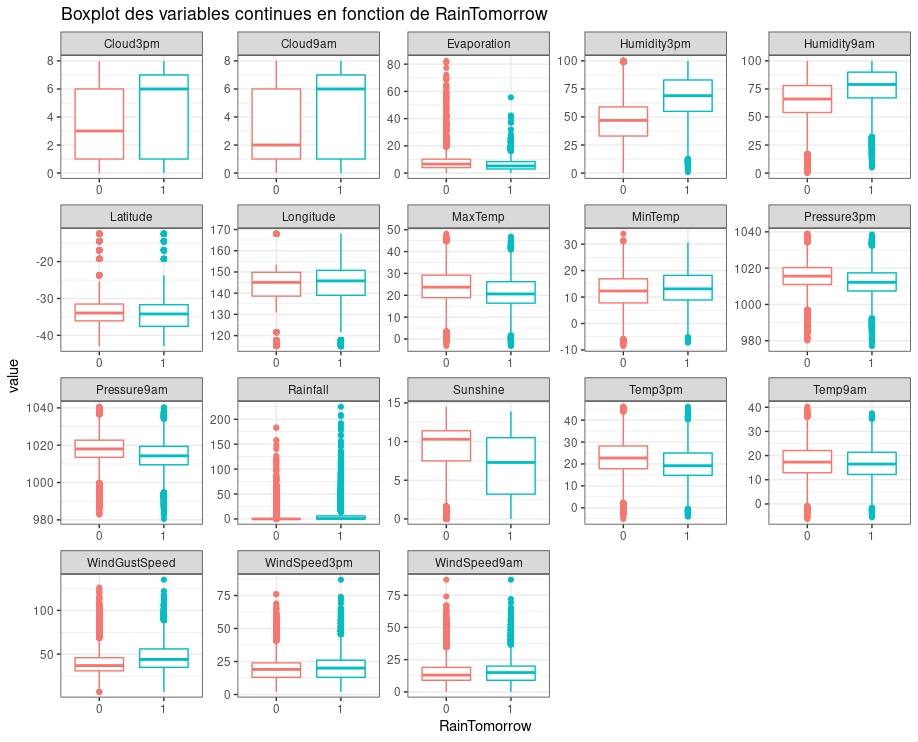
\includegraphics[width=0.7\textwidth]{Images/boxplots/boxplot_RainTomorrow.png}
    \caption{Boxplots pour la variable RainTomorrow}
    \label{fig:bp_raintomorrow}
\end{figure}

Jetons maintenant un coup d'oeil aux boîtes des variables RainToday (Figure \ref{fig:bp_raintoday}) et RainTomorrow (Figure \ref{fig:bp_raintomorrow}). Comme on peut s'y attendre elles sont très similaires. En effet, d'un jour au lendemain, il n'y a pas de changement énorme. Comme ces deux variables sont liées (Si RainToday alors RainTomorrow pour le jour d'avant), nous avons ces similarités. Une différence notable est celle des boîtes affichées pour la variable Rainfall : par construction de la variable RainToday, il n'y à pas d'observations ou Rainfall a une valeur supérieure à 0 et ou RainToday est à 1. Ça n'est pas le cas pour RainTomorrow évidemment, il y aura toujours un moment ou il pleut aujourd'hui mais il ne pleuvra pas demain (sinon la pluie ne s'arrêterait jamais).

Comme on peut s'y attendre, les variables d'humidité sont plus elevée lorsqu'il pleut (RainToday). On peut voir cependant ces mêmes différences pour RainTomorrow, avec quelques variations : l'humidité à 15h et à 9h est plus elevée lorsqu'il pleut le lendemain (cette différence est surtout notable pour Humidity3pm, les distances inter-quartiles ne se chevauchent presque pas).

\part{Prédiction}

Maintenant que notre base de données est prête que nous la connaissons plus en détail, nous pouvons commencer à créer nos modèles de prédiction. Commençons tout d'abord par faire une analyse en composantes principales, pour avoir une meilleure idée de la distribution des observations.

\section{ACP}

Rappelons tout d'abord la distribution des observations où il pleut le lendemain et où il ne pleut pas : 

\begin{table}[H]
    \centering
        \begin{tabular}{|rrr|}
            \hline
            RainTomorrow & Compte & \% \\ 
            \hline
            \hline
            0 & 82367 & 78.04 \\
            1 & 23179 & 21.96 \\
            \hline
        \end{tabular}
    \caption{Distribution des valeurs de la variable RainTomorrow dans nos données finales.}
\end{table}

Et lorsque l'on affiche une analyse en composantes principales de ces observations, et en les colorant en fonction de leur valeur de RainTomorrow, on obtient le graphique de la Figure \ref{fig:pca_raintomorrow}.

\begin{figure}[htp]
    \centering
    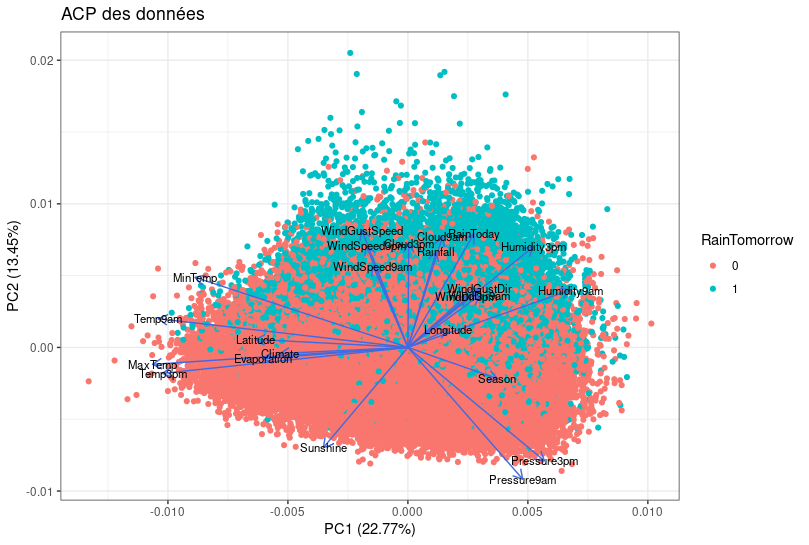
\includegraphics[width=0.8\textwidth]{Images/pca.png}
    \caption{Analyse en Composantes Principales de nos données, points colorés en fonction de RainTomorrow.}
    \label{fig:pca_raintomorrow}
\end{figure}

Nous allons donc chercher un moyen de séparer ces deux groupes pour faire des prédictions. On voit déjà (avec 44.06\% de l'information, l'axe 1 représentant 27.94\% et l'axe 2 16.12\%) que les observations pour lesquelles il pleut le lendemain sont un peu séparées de celles ou il ne pleut pas. On voit d'ailleurs bien le déséquilibre de nos données sur ce graphique.

On peut noter par ailleurs que les variables d'humidité et les nuages sont importantes pour différencier ces deux groupes. En effet les valeurs de ces variables sont plus élevées pour RainTomorrow = 1. A l'inverse, lorsque la valeur de Sunshine est élevée on va plutôt vers le groupe RainTomorrow = 0. On peut aussi s'amuser à regarder les 2 composantes principales suivantes pour avoir un autre point de vue (on a cette fois-ci 28.51\% de l'information, Figure \ref{fig:pca_raintomorrow2}).

\begin{figure}[htp]
    \centering
    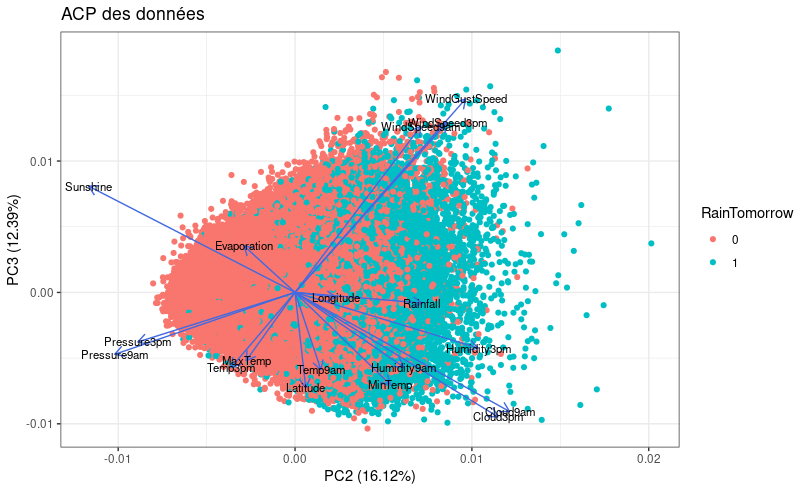
\includegraphics[width=0.8\textwidth]{Images/pca2.png}
    \caption{Analyse en Composantes Principales de nos données, axes 2 et 3, points colorés en fonction de RainTomorrow.}
    \label{fig:pca_raintomorrow2}
\end{figure}

Il semble aussi que les variables de pression sont importantes pour différencier ces deux groupes. 

\section{Premières prédictions}

Dans cette partie nous allons prendre telle quelle la base de données, sans nous soucier de son déséquilibre. Nous allons mettre en place plusieurs modèles de prédiction : 
\begin{itemize}
    \item Un modèle de régression linéaire
    \item Un arbre CART
\end{itemize}

\subsection{Régression linéaires logistique}

\newpage
\printbibliography

\end{document}
